\documentclass[11pt,letterpaper]{article}
\input{headings}
\newcommand \recipeName {Sauteed Salted Potatoes}
\newcommand \fileName {SaltedPotatoes}
\chead{\recipeName}

\begin{document}
\input{title}

This is my adaptation of \href{https://www.cookscountry.com/recipes/7126-roasted-salt-and-vinegar-potatoes?extcode=MCSKD10L0&ref=new_search_experience_1}{Cook's Country Roasted Salt-and-Vinegar Potatoes}. We cooked that recipe a couple of times and then we decided that we did not like the vinegar. Also, I found that it is easier, and it also produces better results, to sautee the potatoes instead of roasting them after they are flatenned. I also had to do this recipe for a crowd, thus I came up with a faster way to flatten the potatoes while ensuring that they all have the same thickness.

\begin{description}

\item[Ingredients:]\ \\
	\begin{itemize}
	\item 2 pounds of small potatoes
	\item 1 1/4 cup of salt
	\item 6 tablespoons of olive oil
	\item freshly grated pepper
	\end{itemize}

\item[Equipment:]\ \\
	\begin{itemize}
	\item Large pot
	\item non-stick skillet
	\item Flat bottom pot or skillet
	\item Serving platter
        \item Baking sheet fitted with a wire rack
        \item Colander
        \item Offset spatula
	\end{itemize}

\item[Procedure:]\ \\
	\begin{enumerate}
	\item {\bf Boil the Potatoes}
	\begin{itemize}
	\item In a large pot, mix the salt with 2 quarts of water until dissolved.
	\item Add the potatoes to the cold salted water and put to cook over moderate high heat.
	\item Dump the potatoes onto the colander inside the sink.
	\item Transfer the potatoes to the wire rack on top of the baking sheet and let the potatoes dry for at least ten minutes. You can boil the potatoes in advance and let then cool and dry completely for a longer time.
	\end{itemize}
	\item {\bf Flatten Potatoes}
	\begin{itemize}
          \item For a small recipe for a Tuesday night supper, you can simply flatten the potatoes individually using the oiled bottom of a metal measuring cup.
	\item For a larger recipe I use two guides and a cold large flat bottom skillet or pot to flatten the potatoes so that they are about 3/4 inch thick. A way that I found to create guides is to use AAA bateries that I join together with packing tape and then wrap around aluminum foil to make it food safe (the guides will not touch the potatoes). You can use other devices of similar thickeness as guides. 
	\item If preparing a larger quantity, oil an area od the counter top.
        \item Place the guides on the edges of the oiled region of the countertop in such a way that they will anchor the bottom of the skillet or pot.
        \item Oil the bottom of the cold pot or skillet.
        \item Place several potaoes in the oiled area of the countertop leaving enough space between them so that they can expand when flatenned.
        \item Press with the oiled pot to flatten the potatoes.
        \item Use the offset spatula to gently lift each potato from the counter top. Either transfer them to an oiled baking sheet or straith to the skillet. 
        \item Repeat the process until you have flattened all the potatoes.          
	\end{itemize}
	\item {\bf Sautee the potatoes}
	\begin{itemize}
        \item Put a heavy bottom serving platter into a 200 F warming oven.
	\item Put a thin film of olive oil in the non-stick skillet and place over moderate high heat.
	\item Place a batch of flattened potatoes into a single layer the skillet and let it cook for several minutes. Shake the pan from time to time to gently slide the potatoes in the pan, but avoid moving them much with a fork or spatula.
        \item Peek under a potato to see if it has browned on the first side.
        \item Once the first side is brown, using two forks or a spatula, gently flip each potato to brown on the other side. 
        \item Remove each sauteed potato from this batch to the warm serving plate and sprinkle with freshly ground black pepper.
        \item Replace the serving plate with the potatoes to the waming oven while cooking the second batch.
        \item Serve warm.
	\end{itemize}
	\end{enumerate}
\end{description}
\begin{table}
\begin{tabular}{cccc}
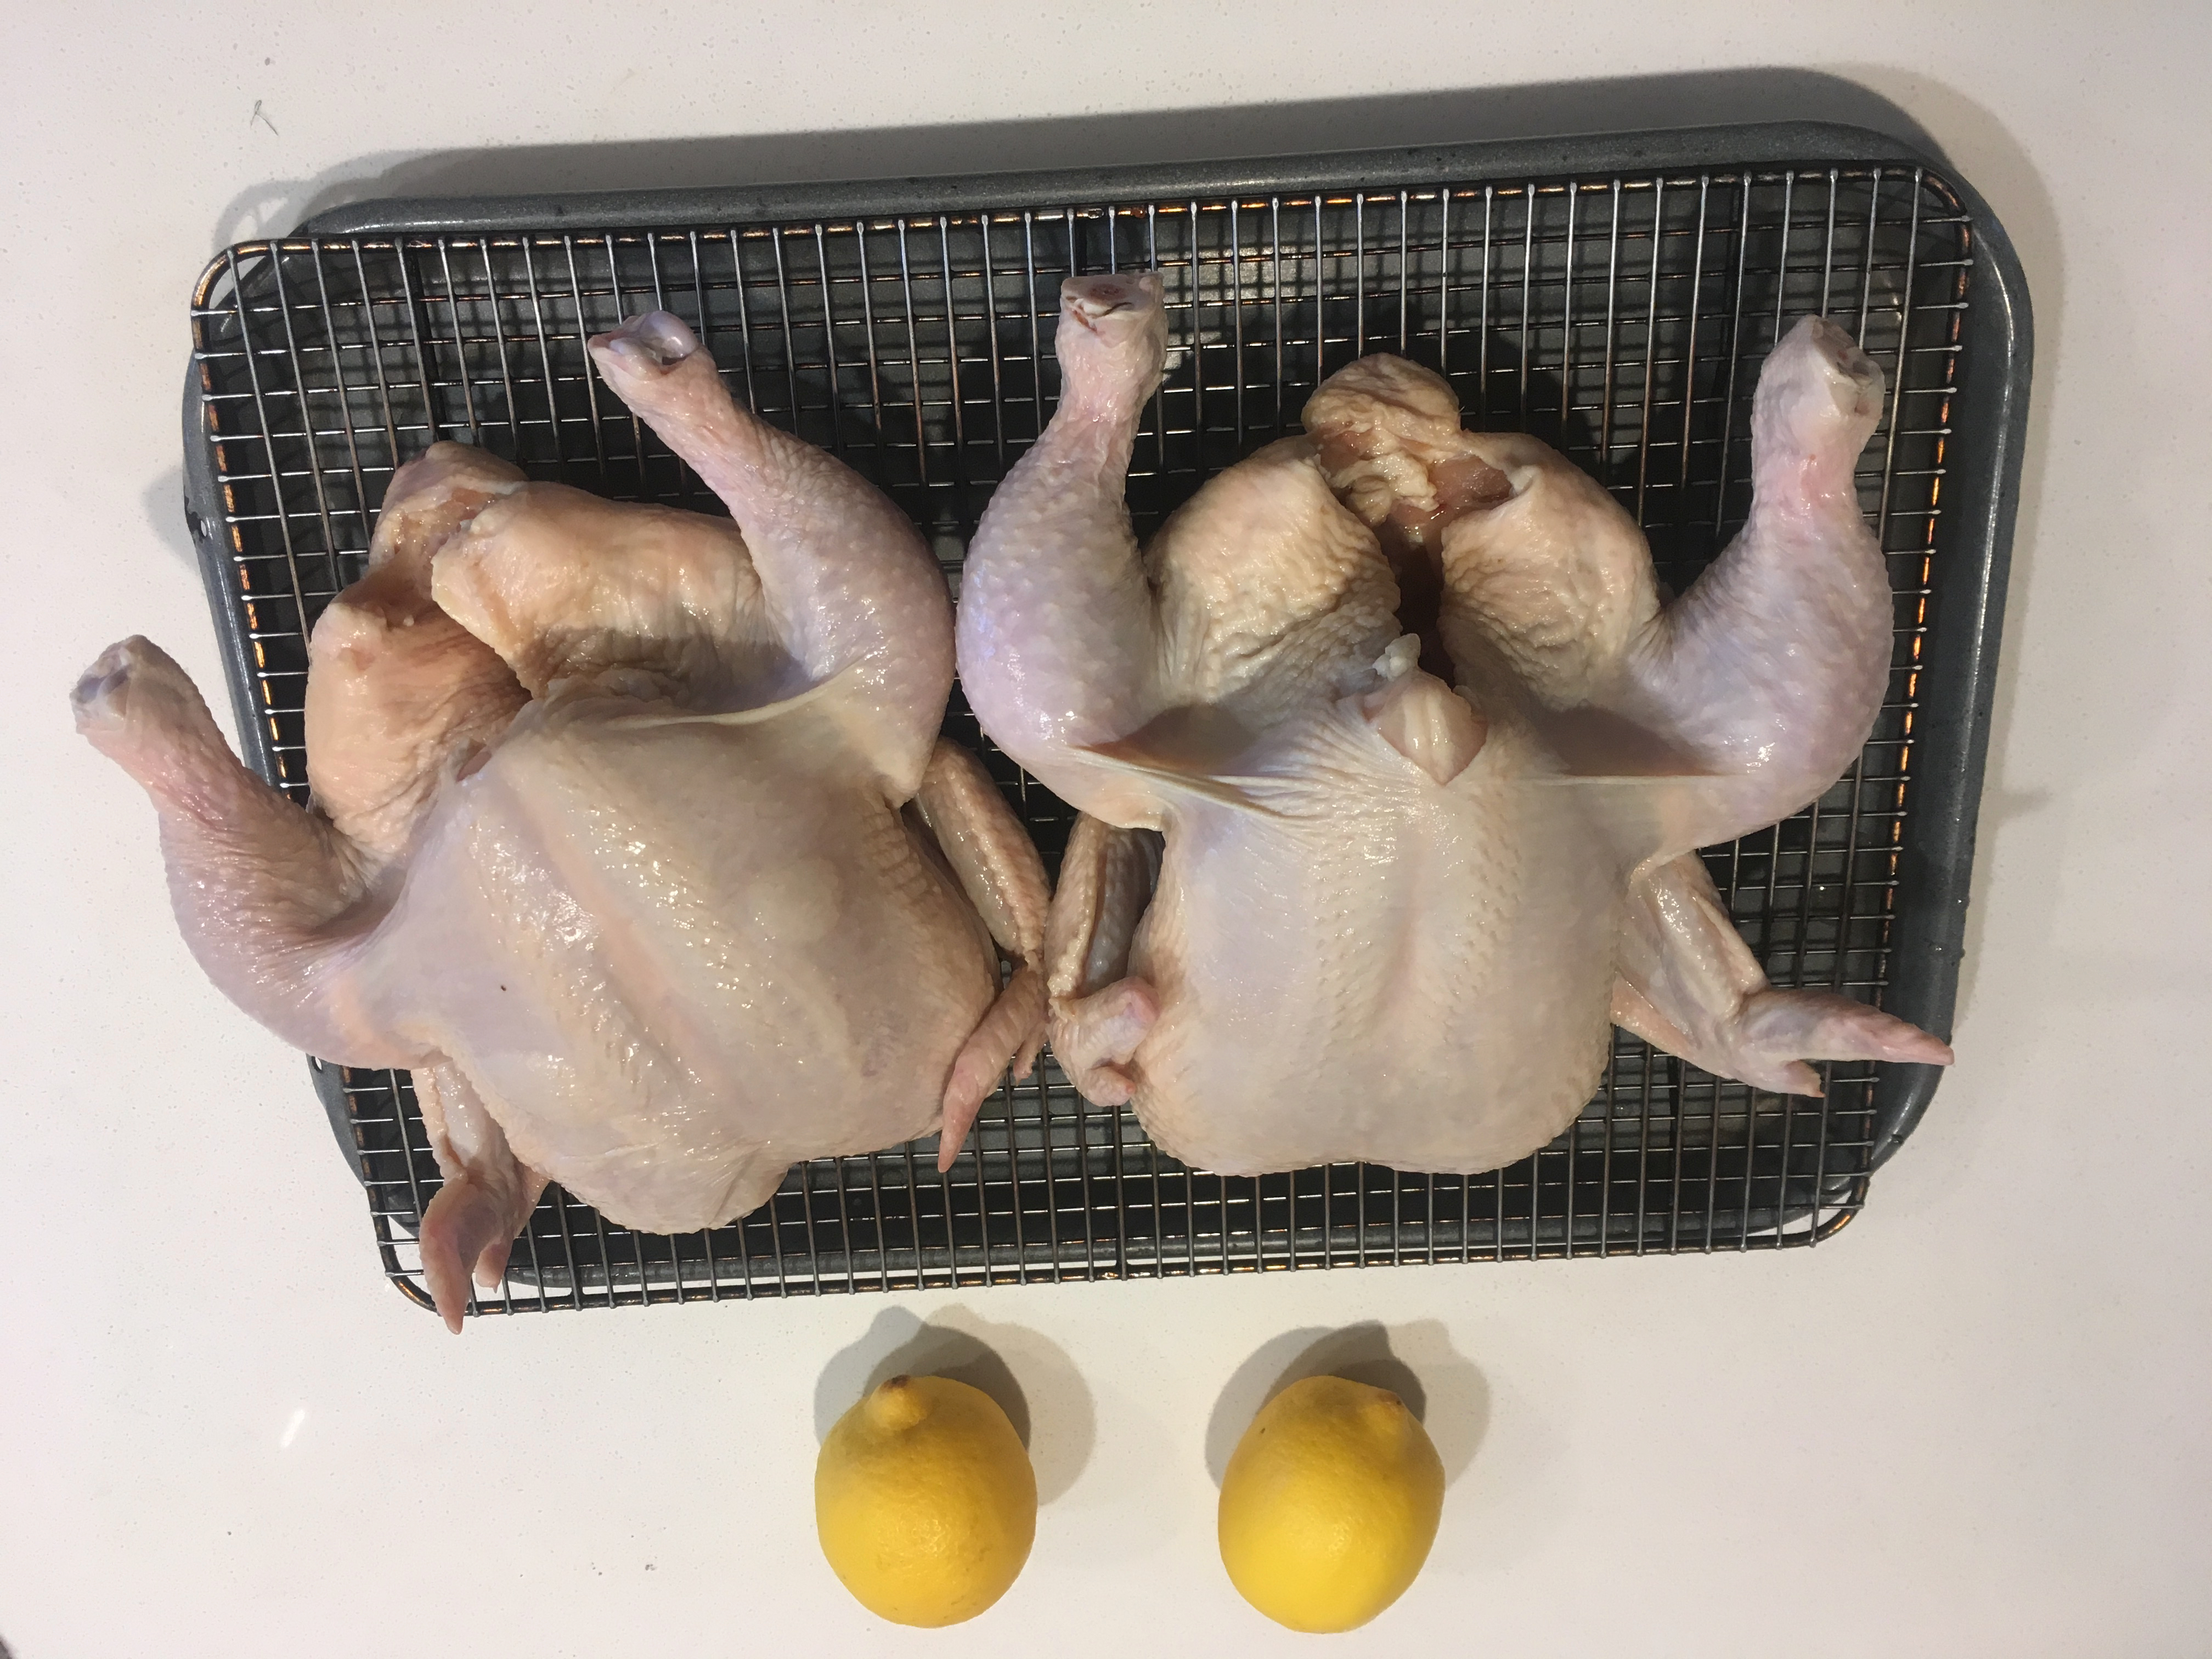
\includegraphics[width=0.25\textwidth]{\imageDir/\fileName/IMG_3197.jpg} &
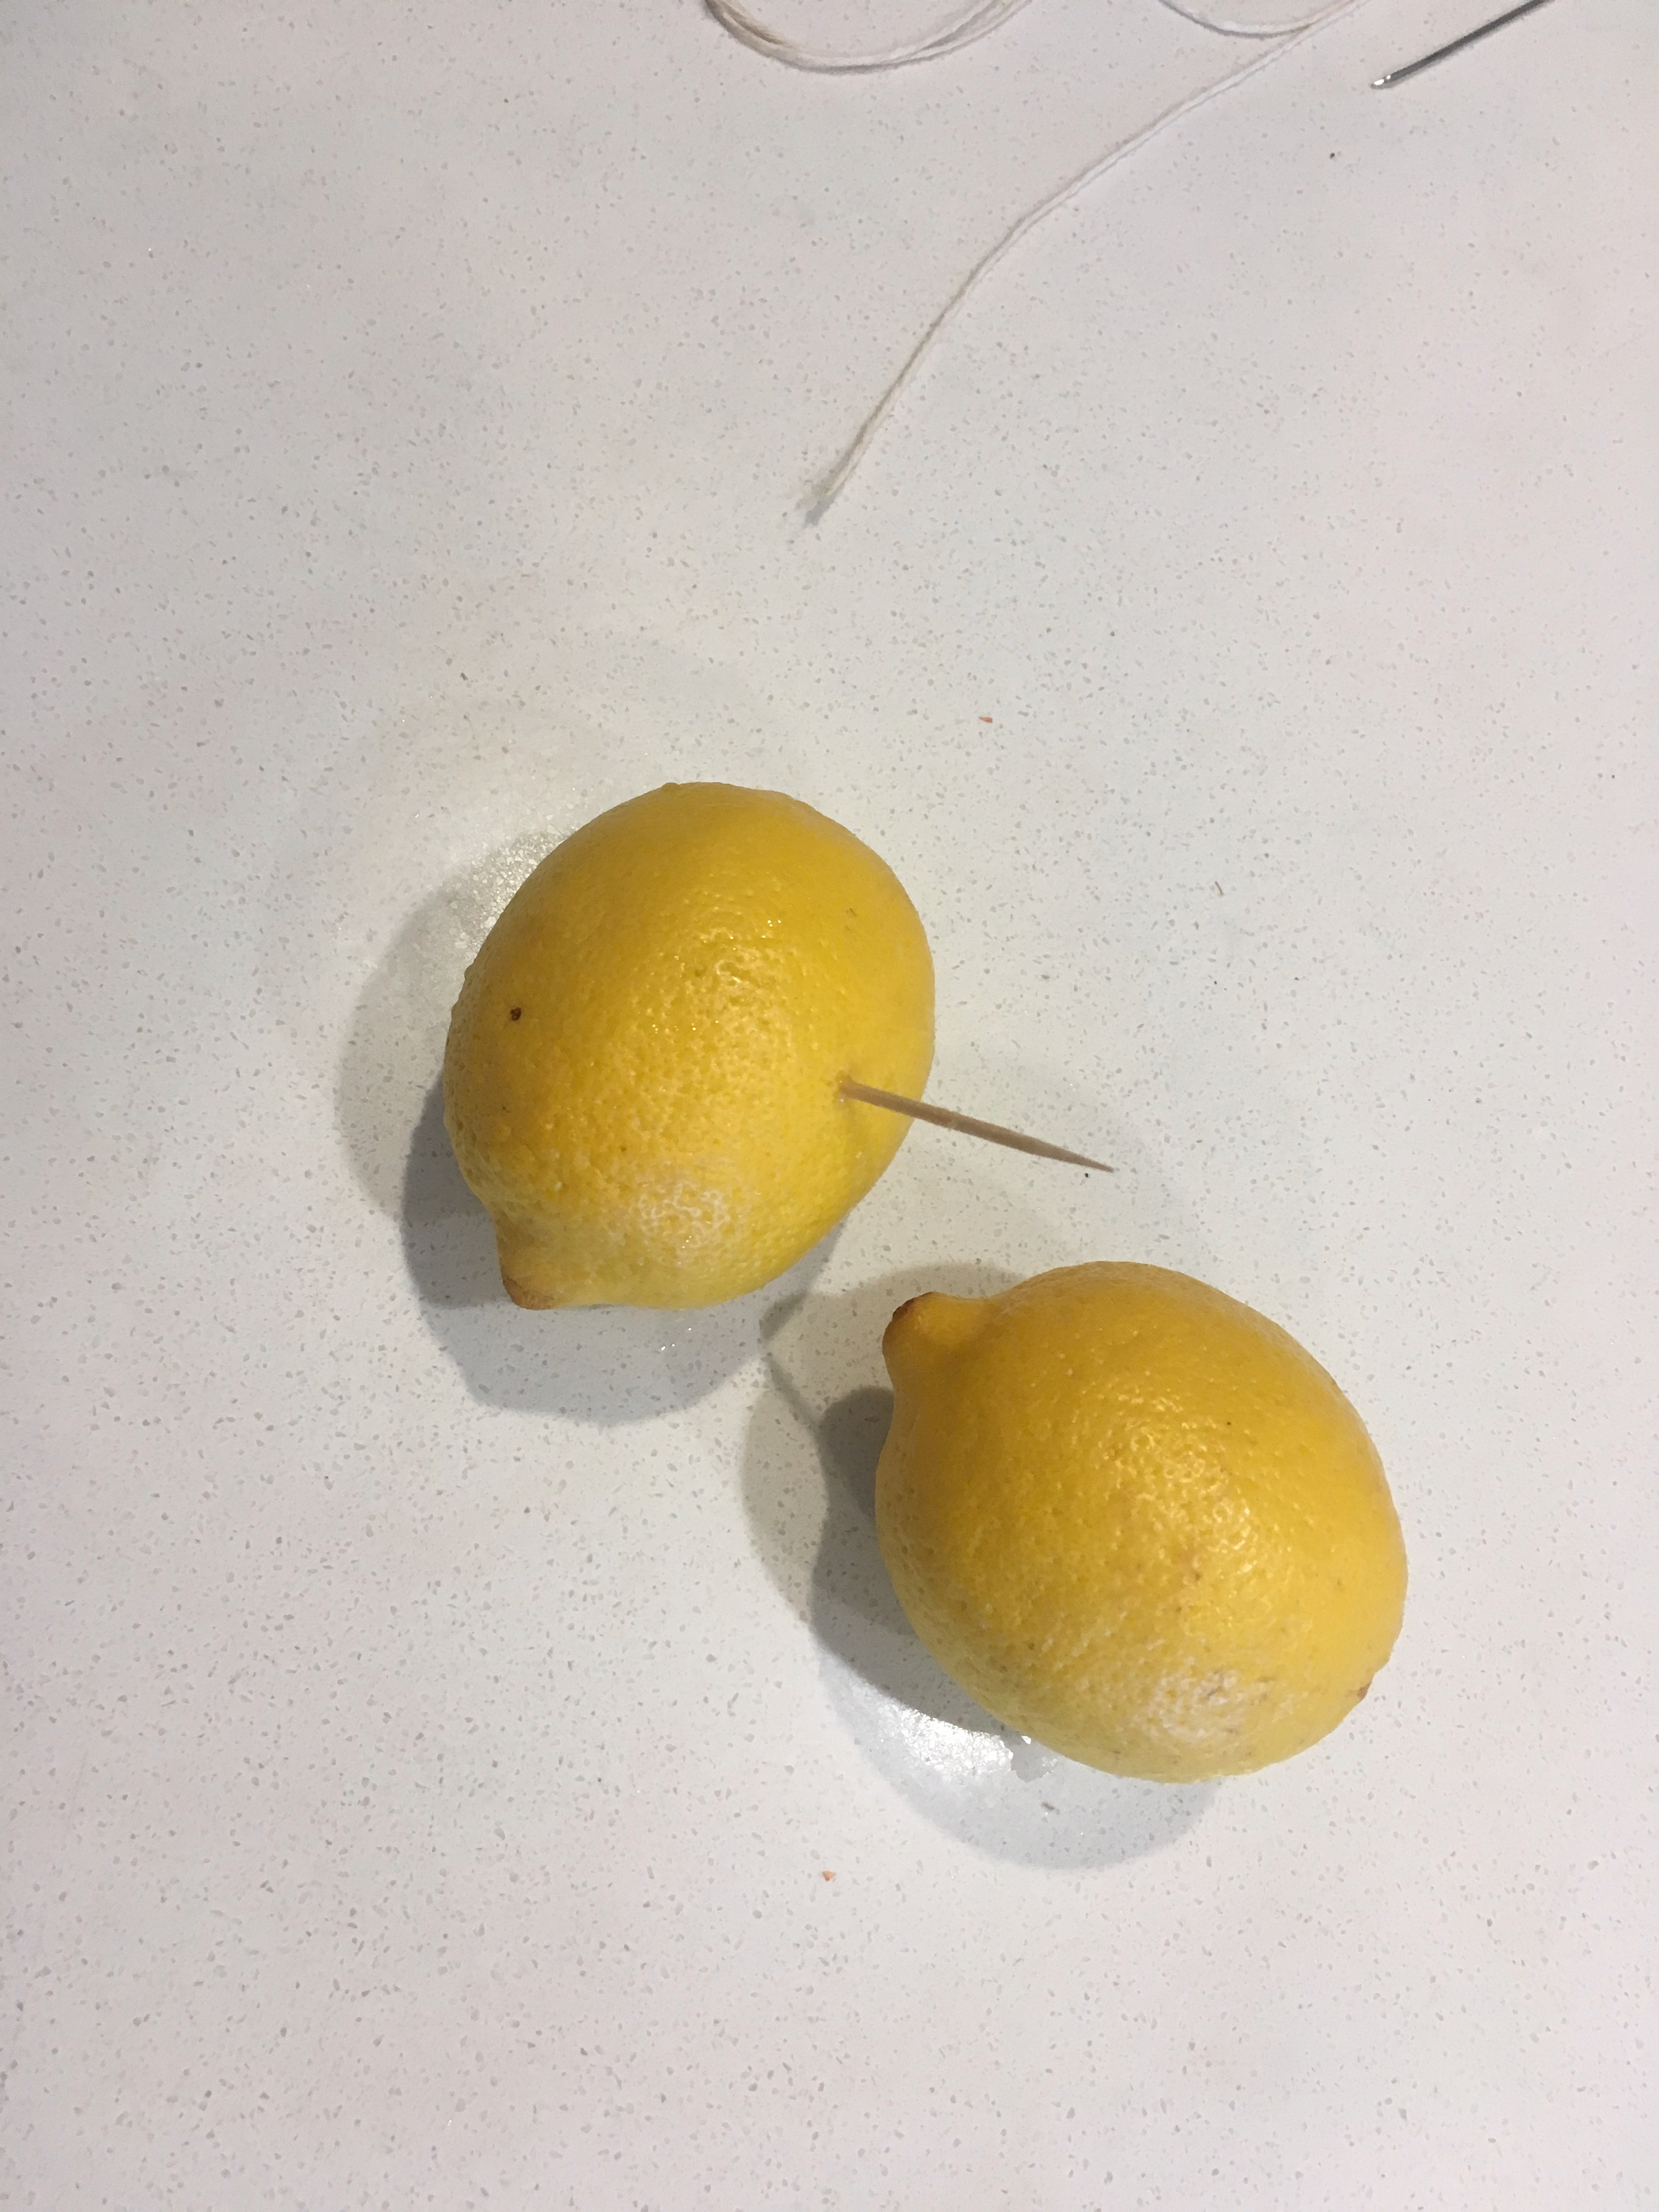
\includegraphics[width=0.25\textwidth]{\imageDir/\fileName/IMG_3212.jpg} &
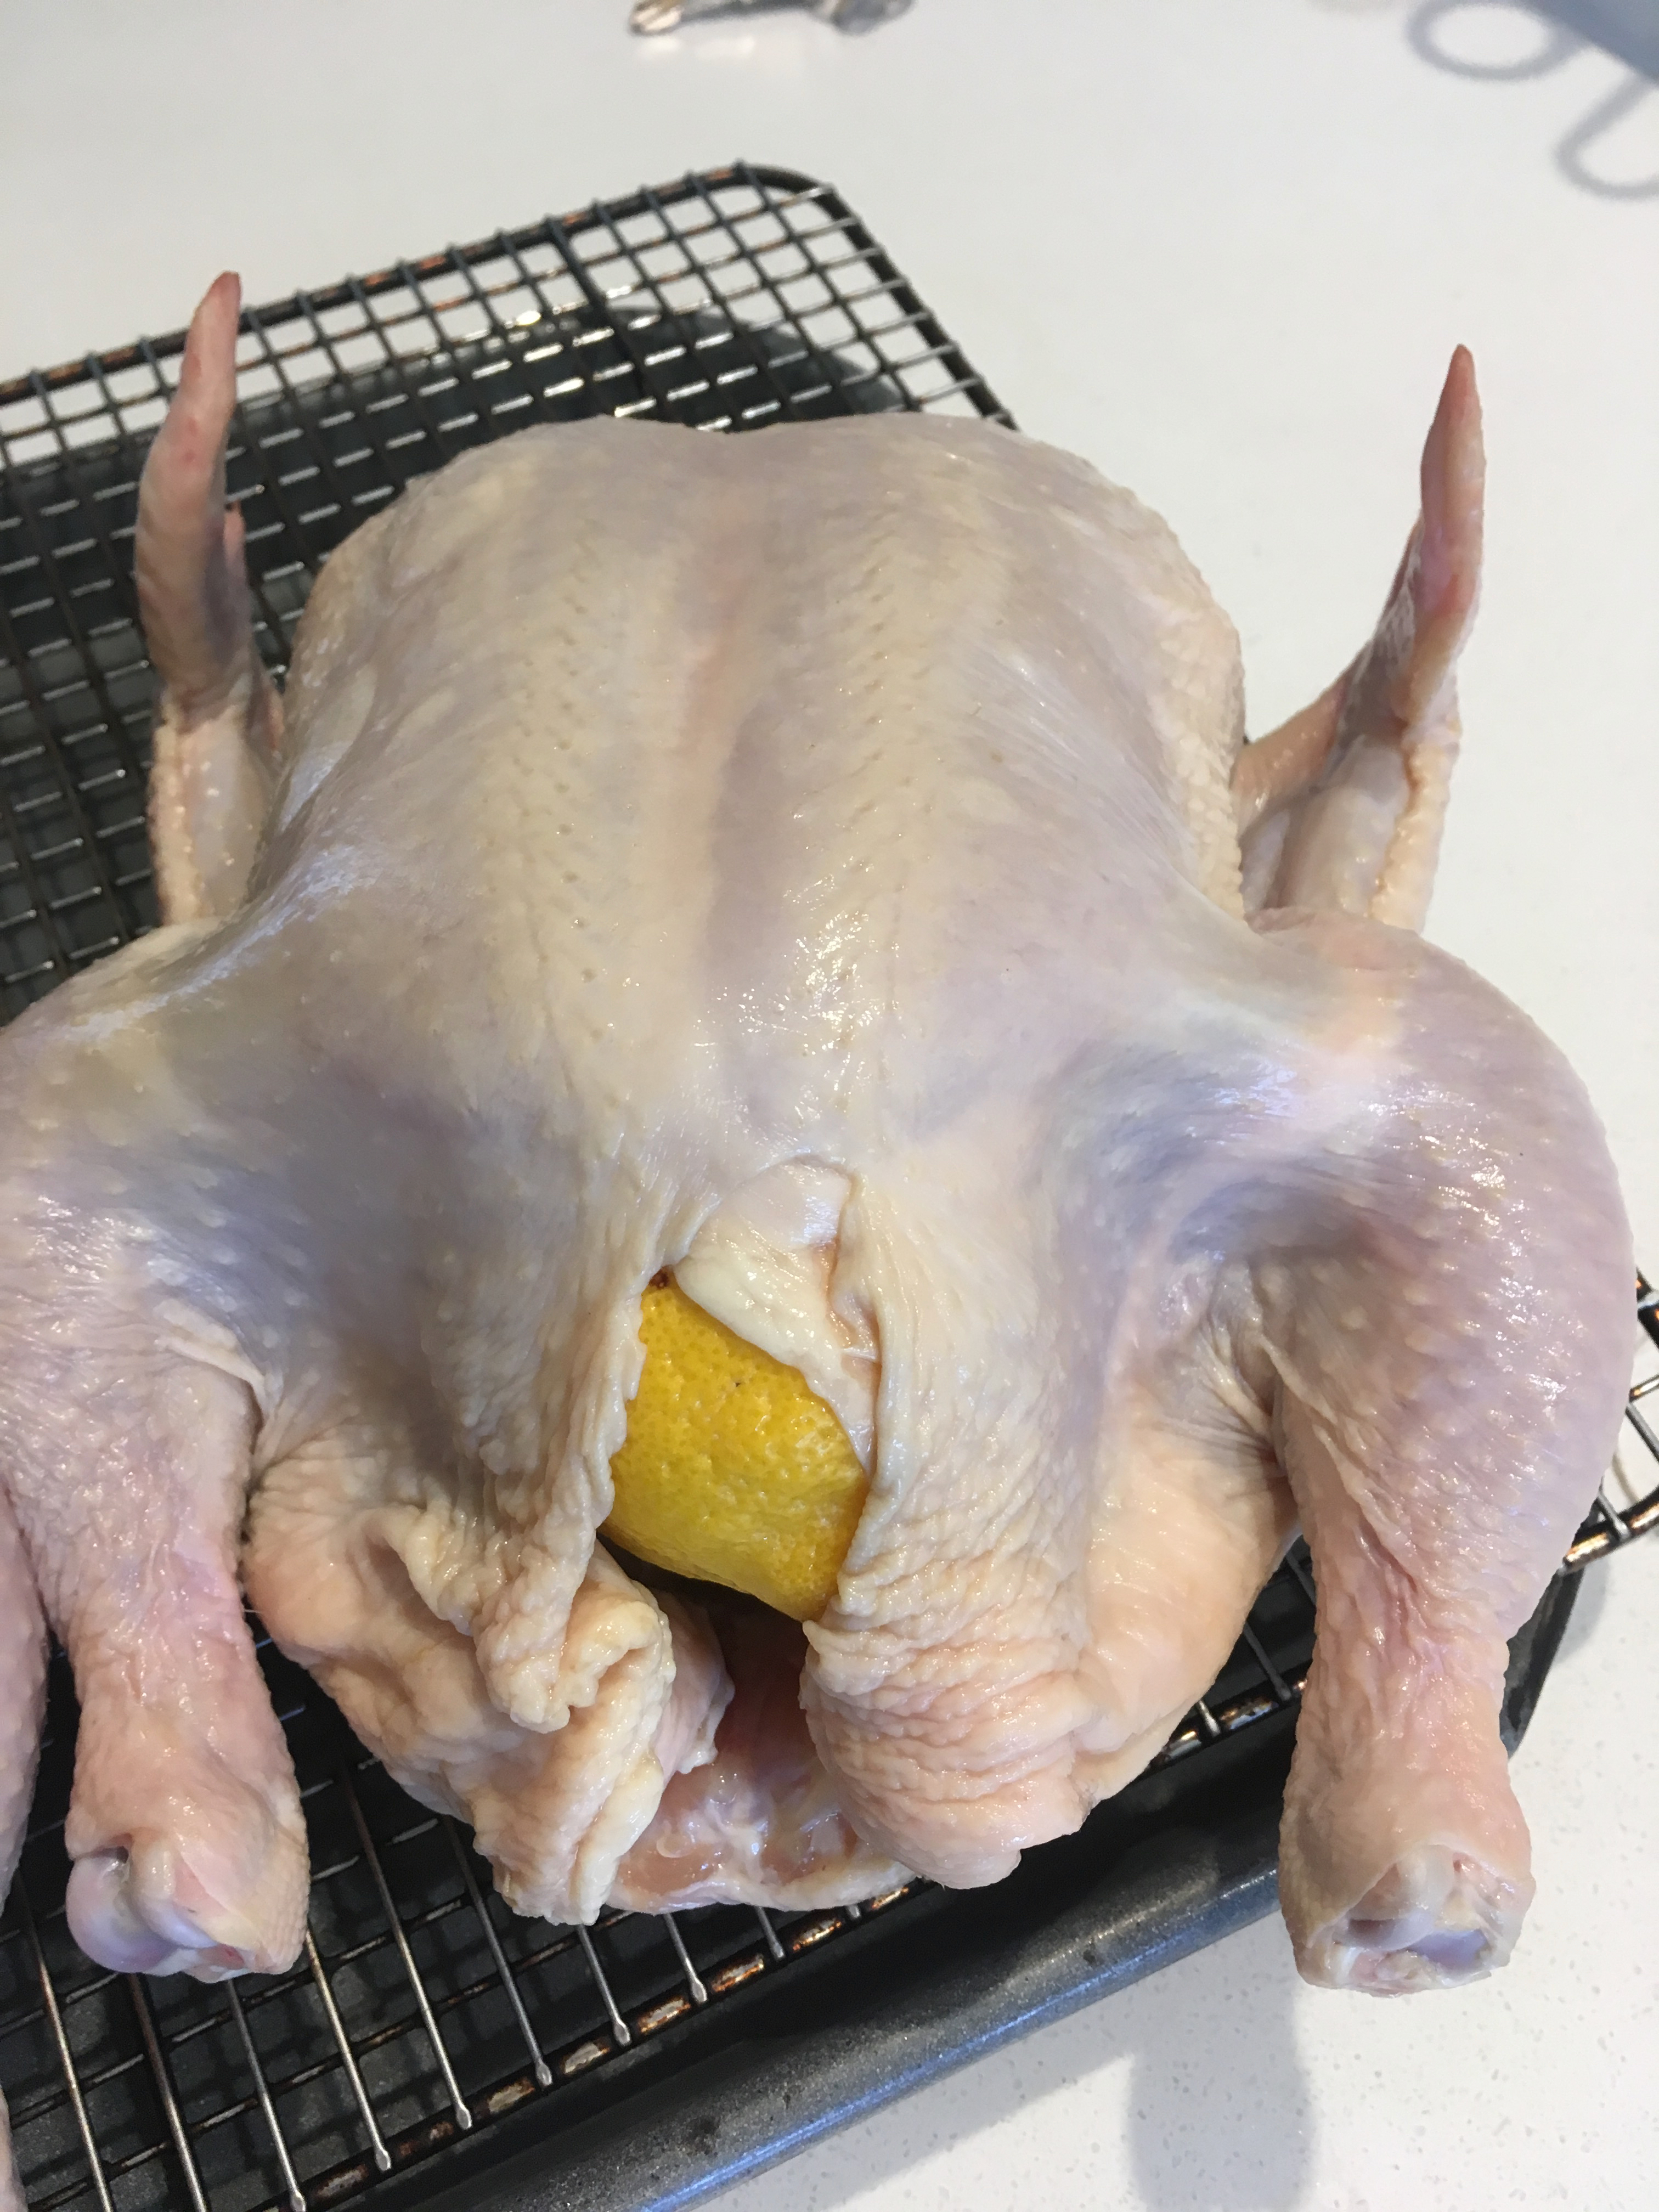
\includegraphics[width=0.25\textwidth]{\imageDir/\fileName/IMG_3213.jpg} \\
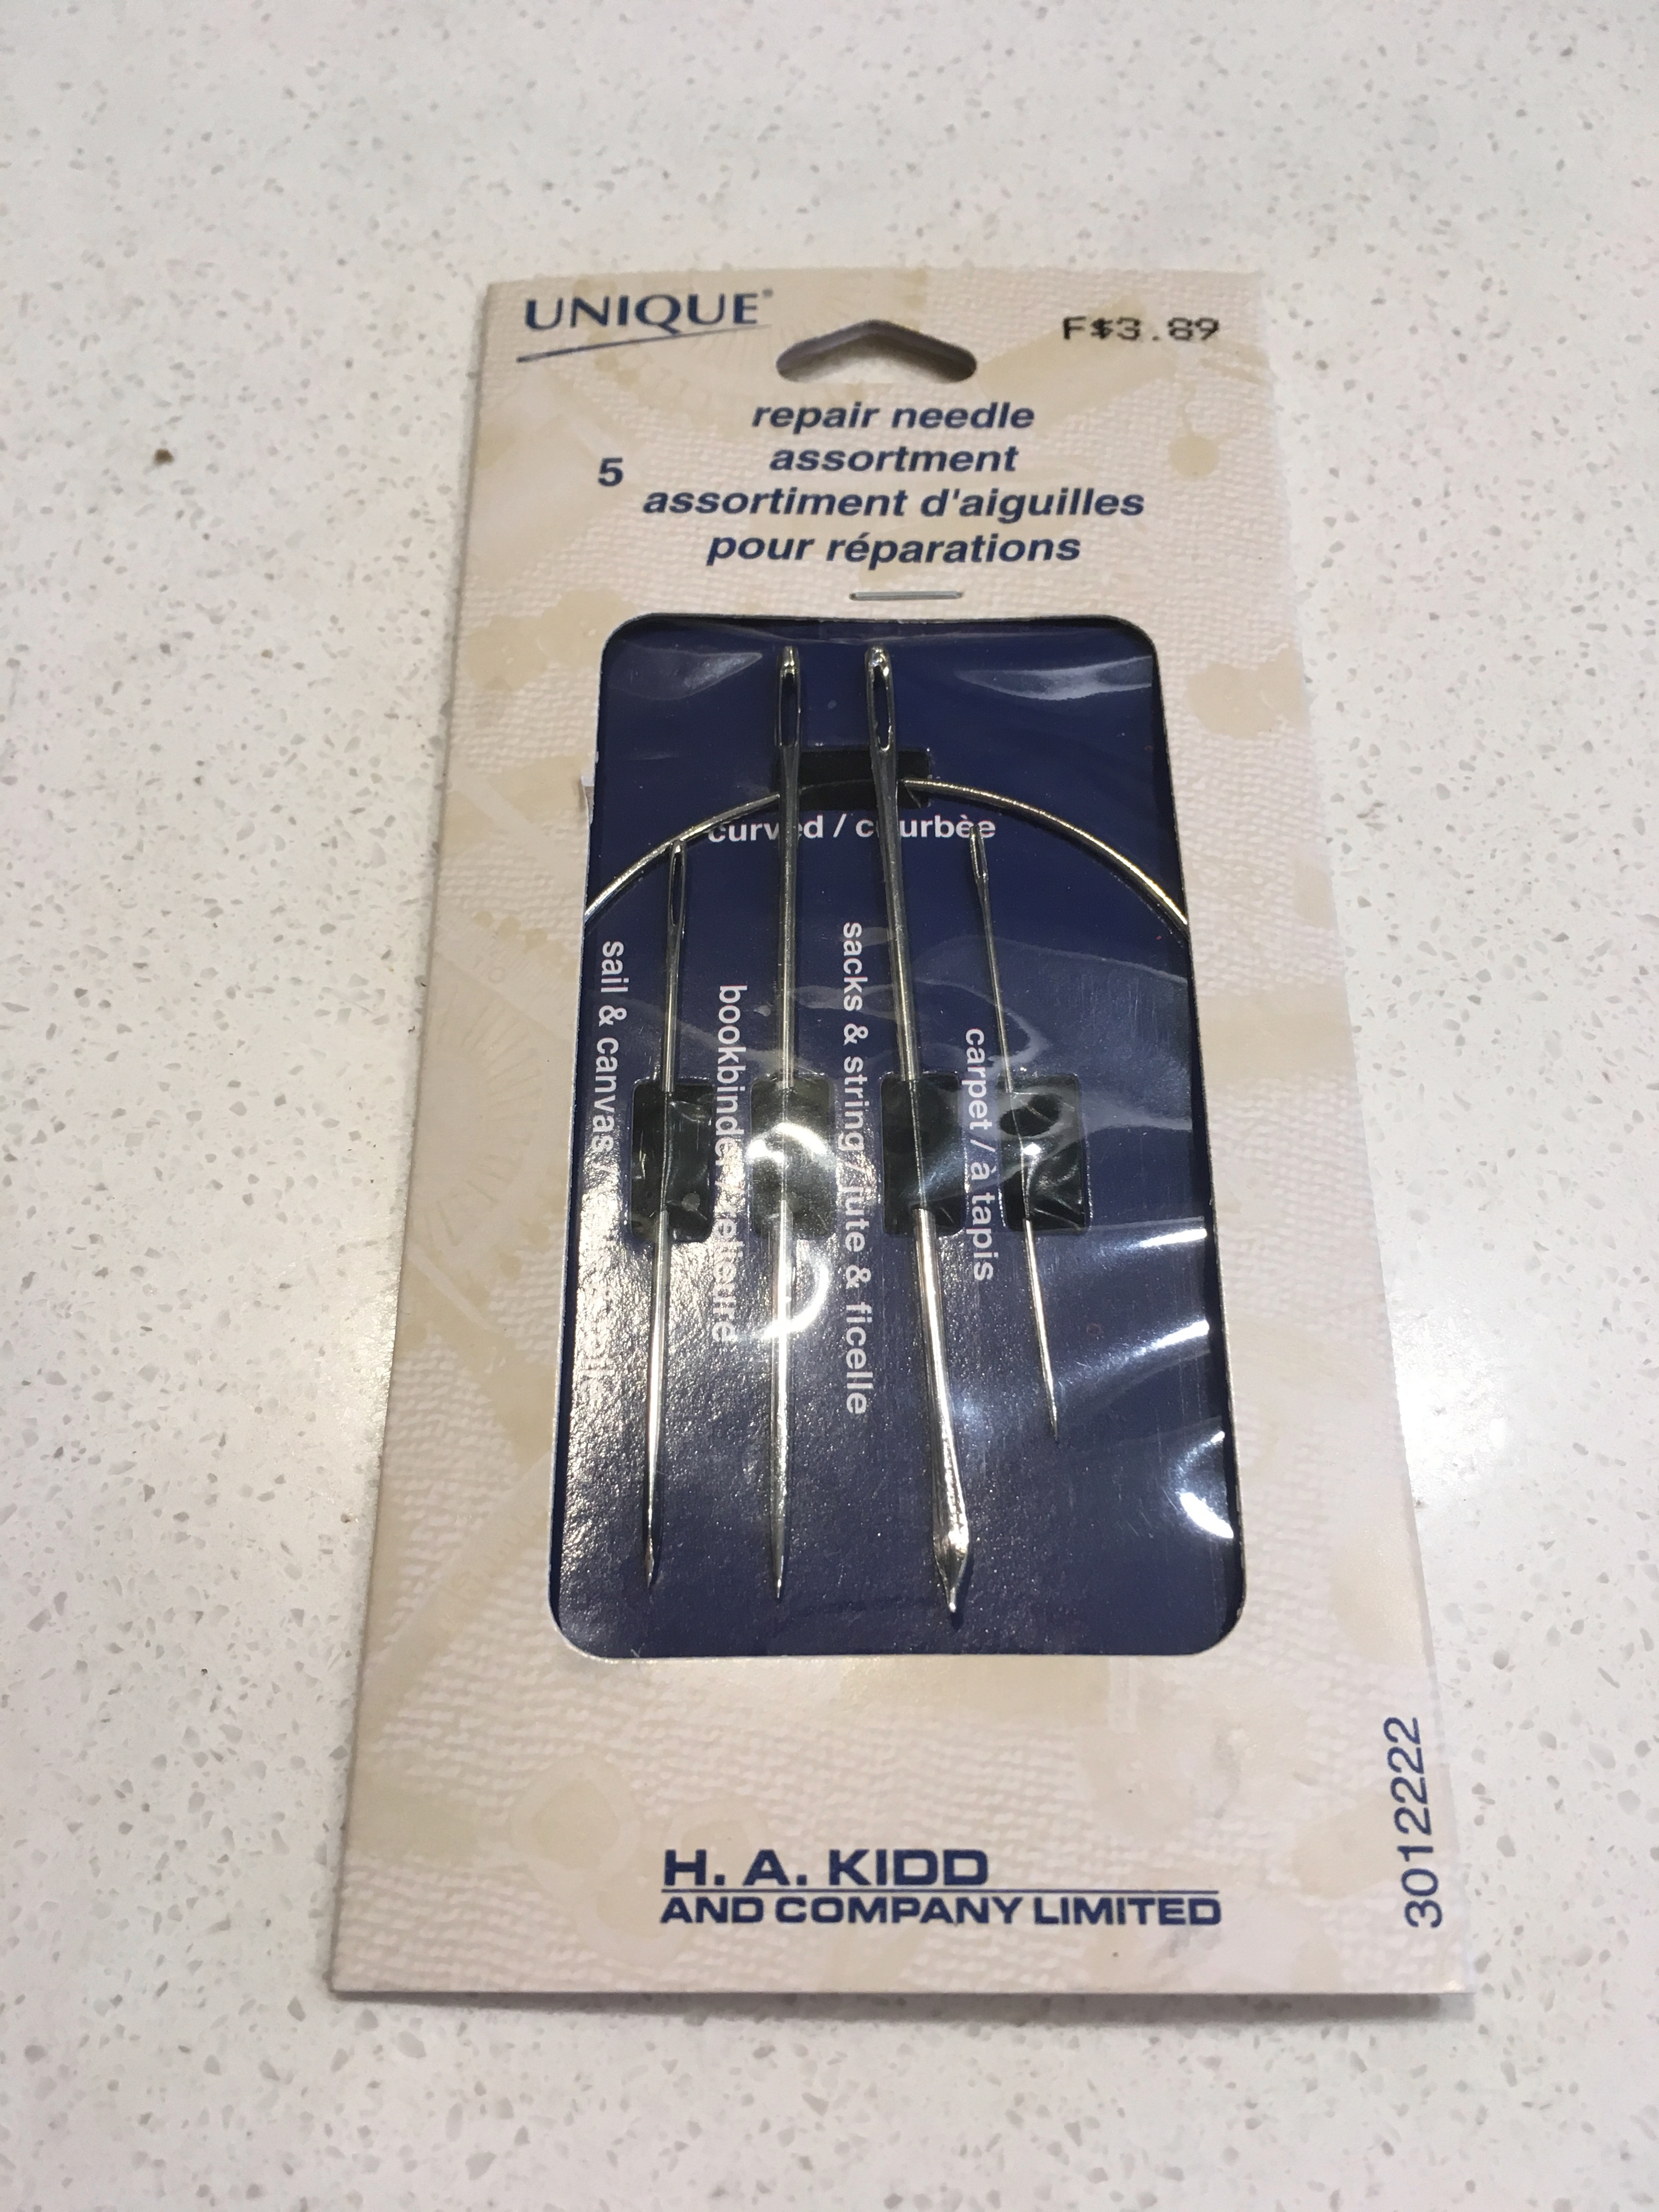
\includegraphics[width=0.25\textwidth]{\imageDir/\fileName/IMG_3206.jpg} &
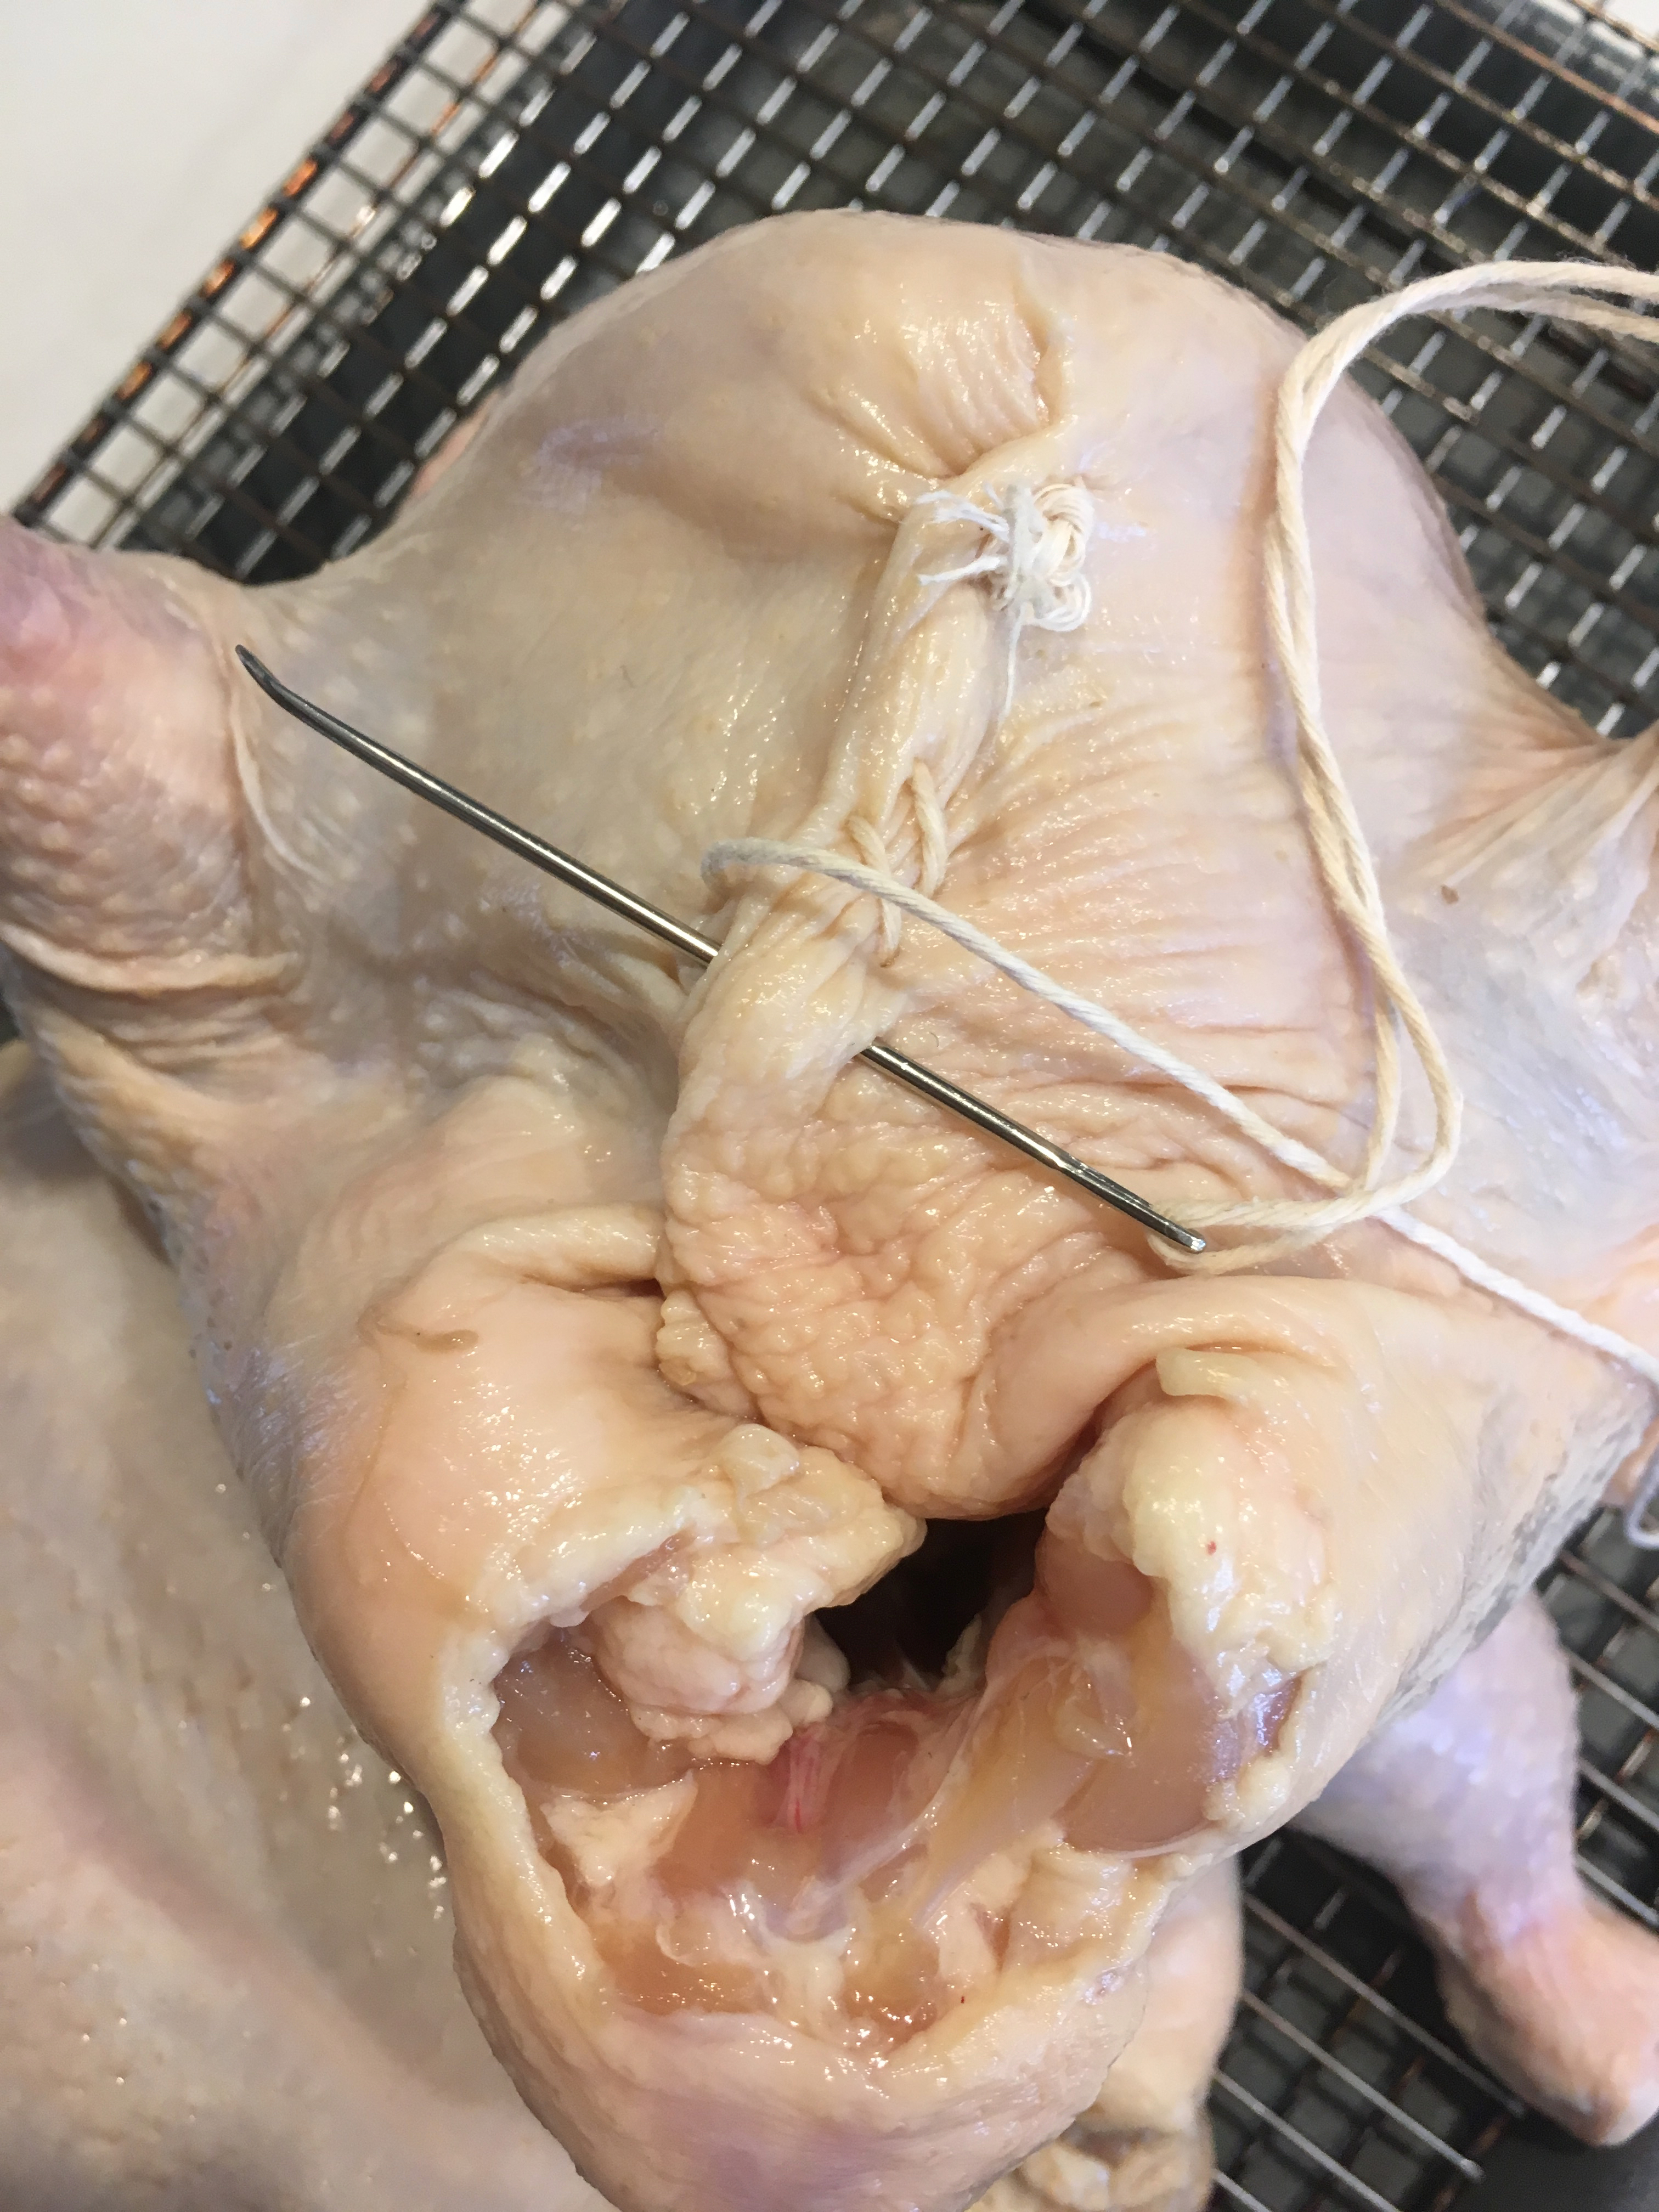
\includegraphics[width=0.25\textwidth]{\imageDir/\fileName/IMG_3214.jpg} &
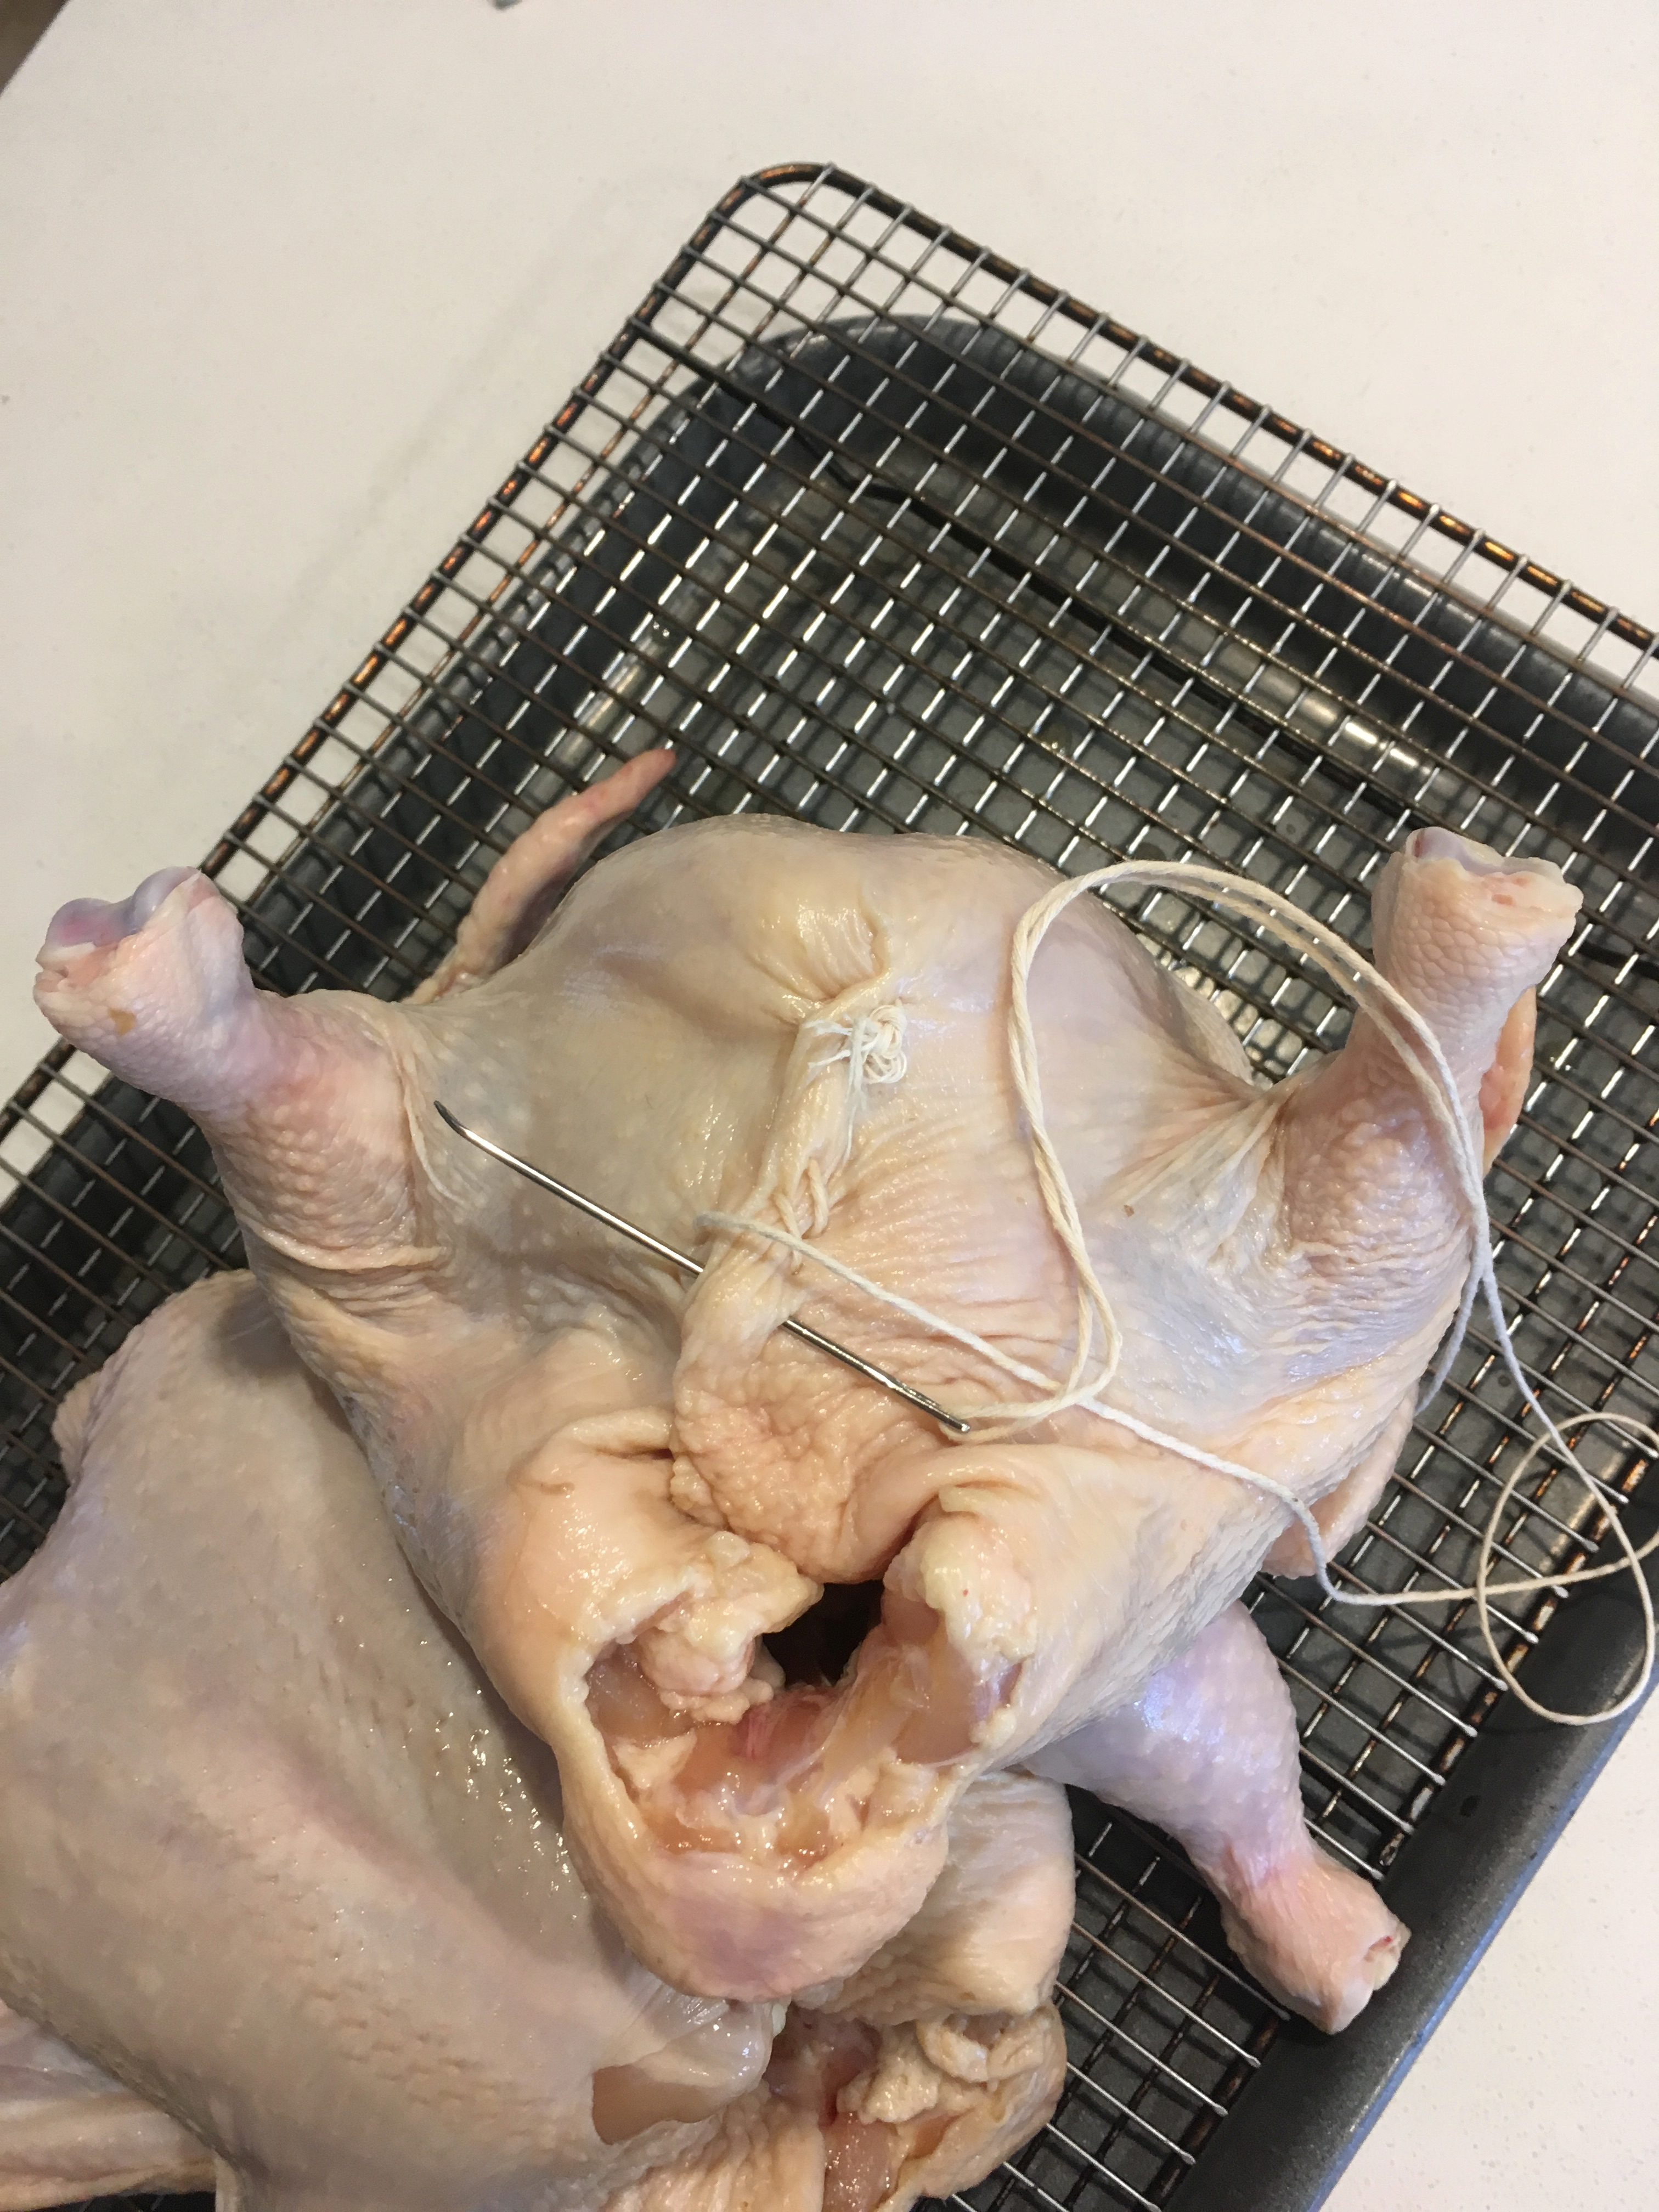
\includegraphics[width=0.25\textwidth]{\imageDir/\fileName/IMG_3216.jpg} \\
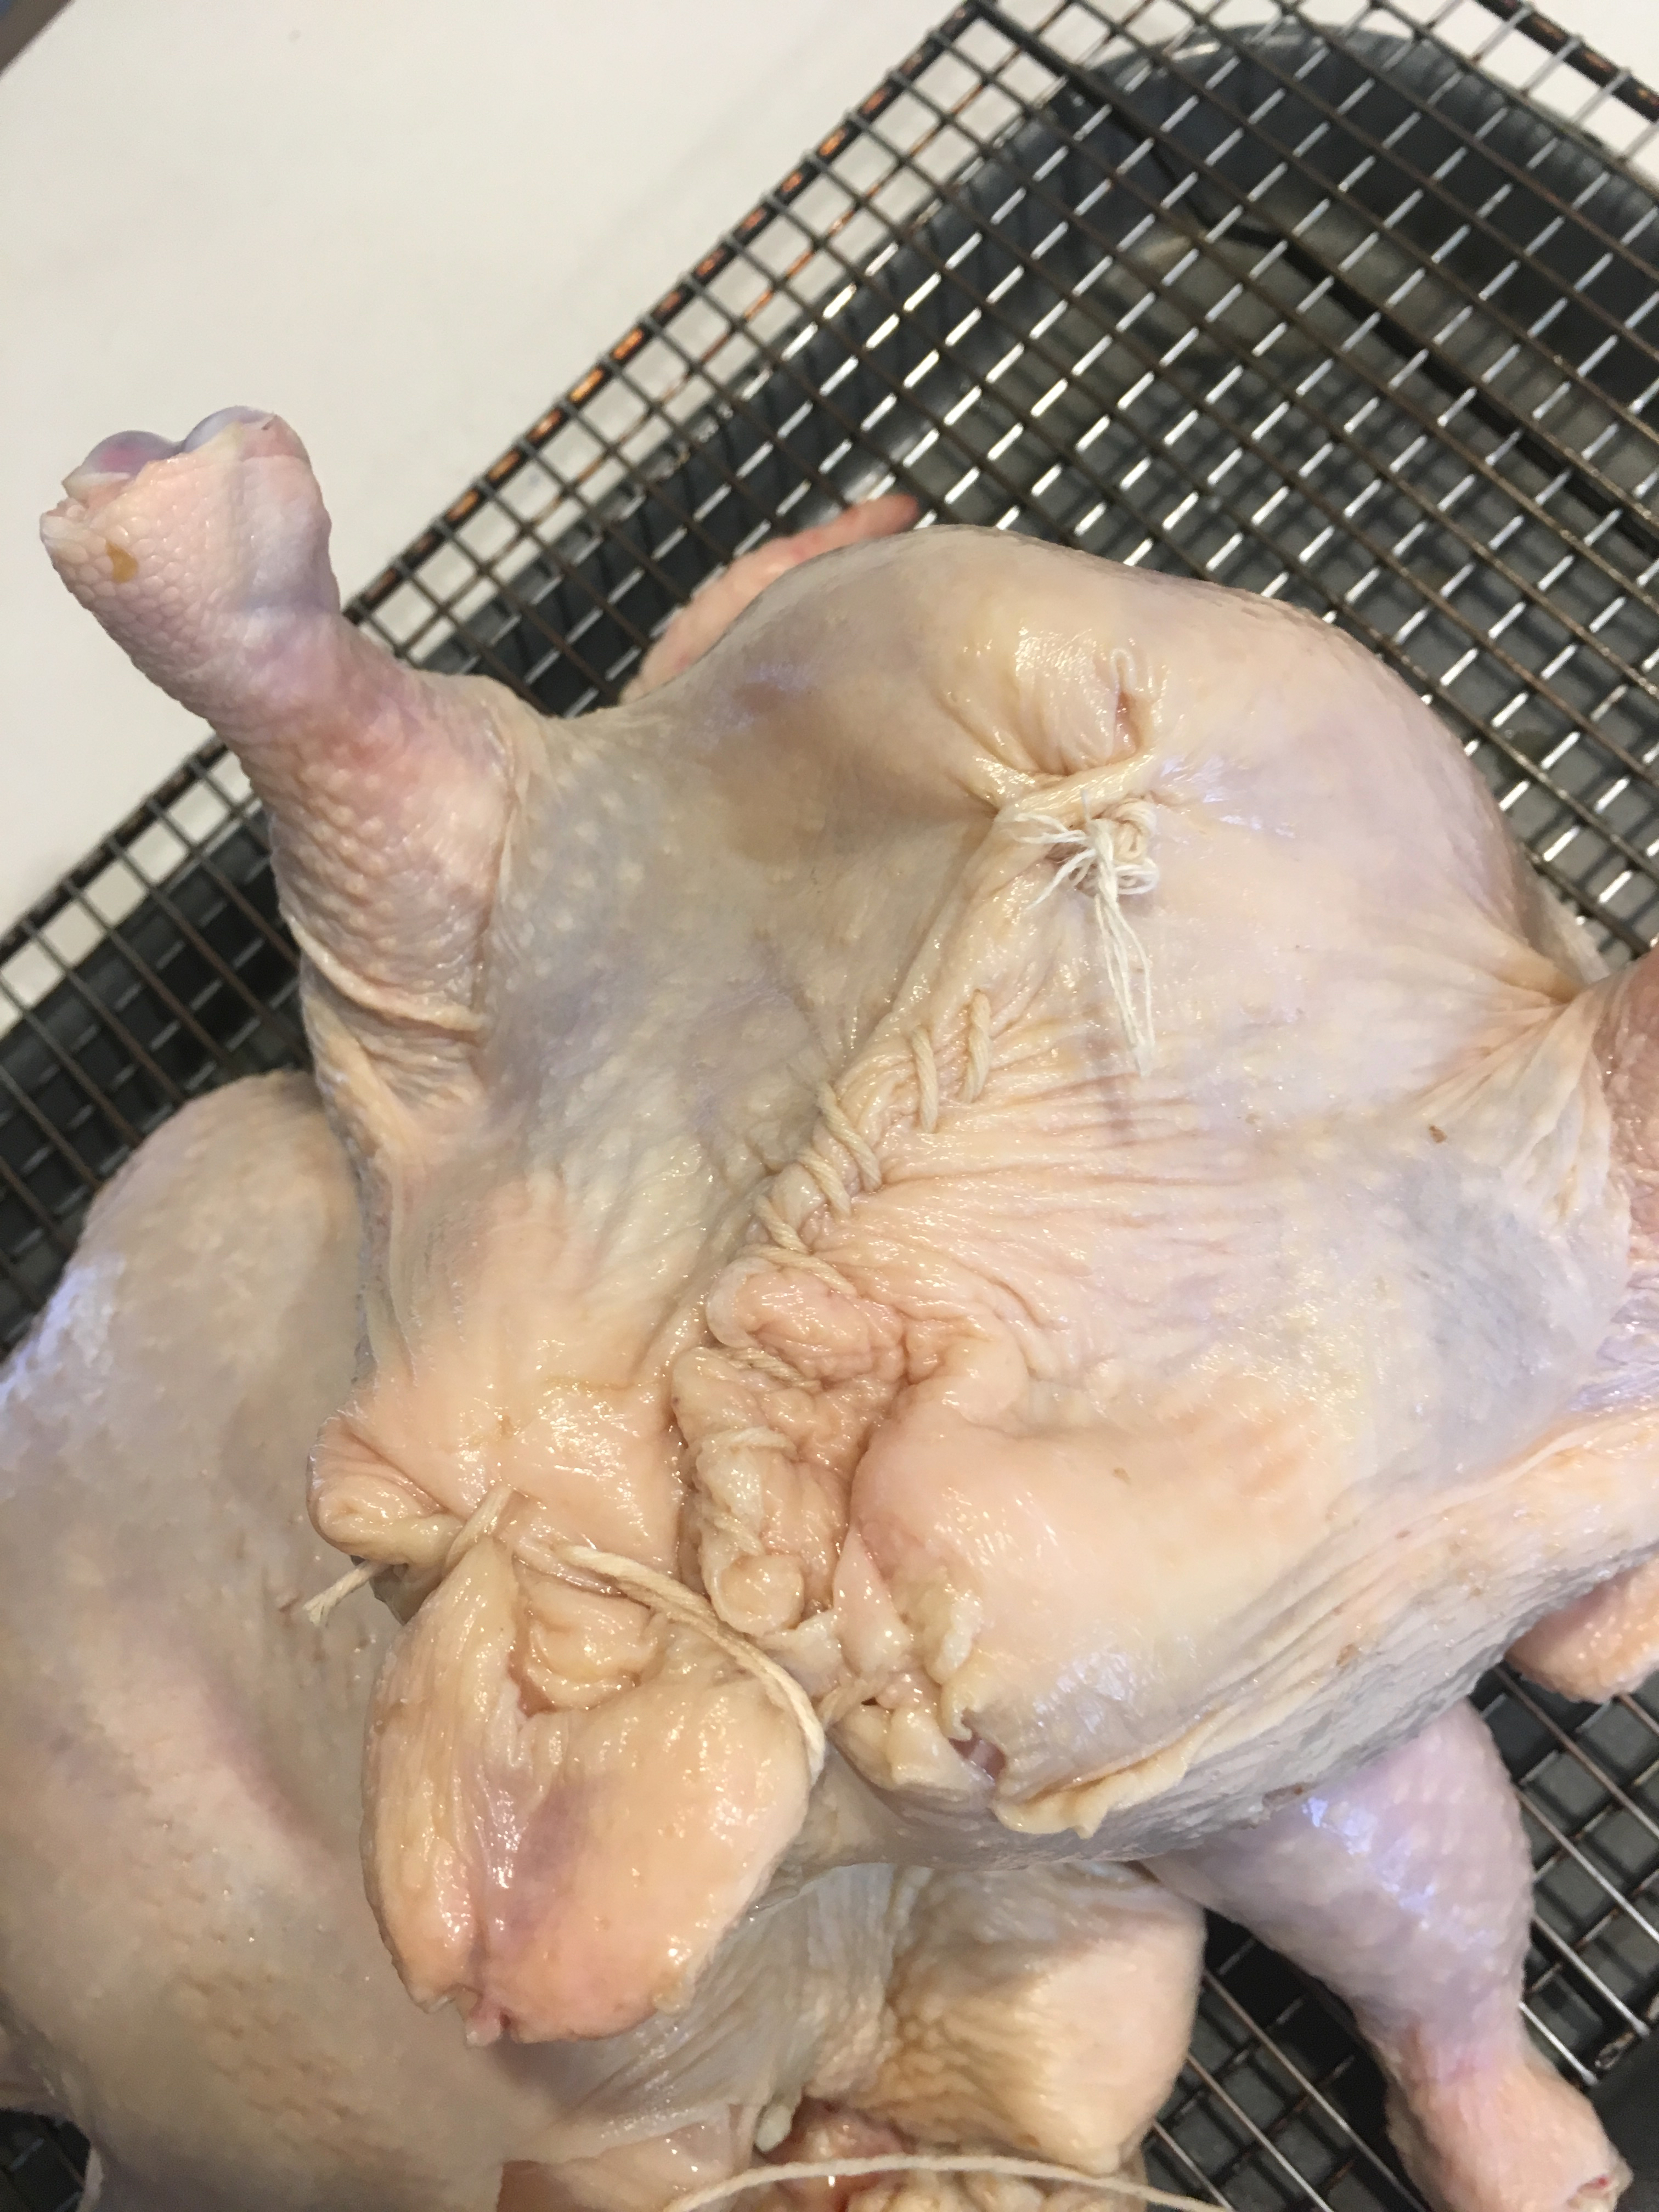
\includegraphics[width=0.25\textwidth]{\imageDir/\fileName/IMG_3217.jpg} &
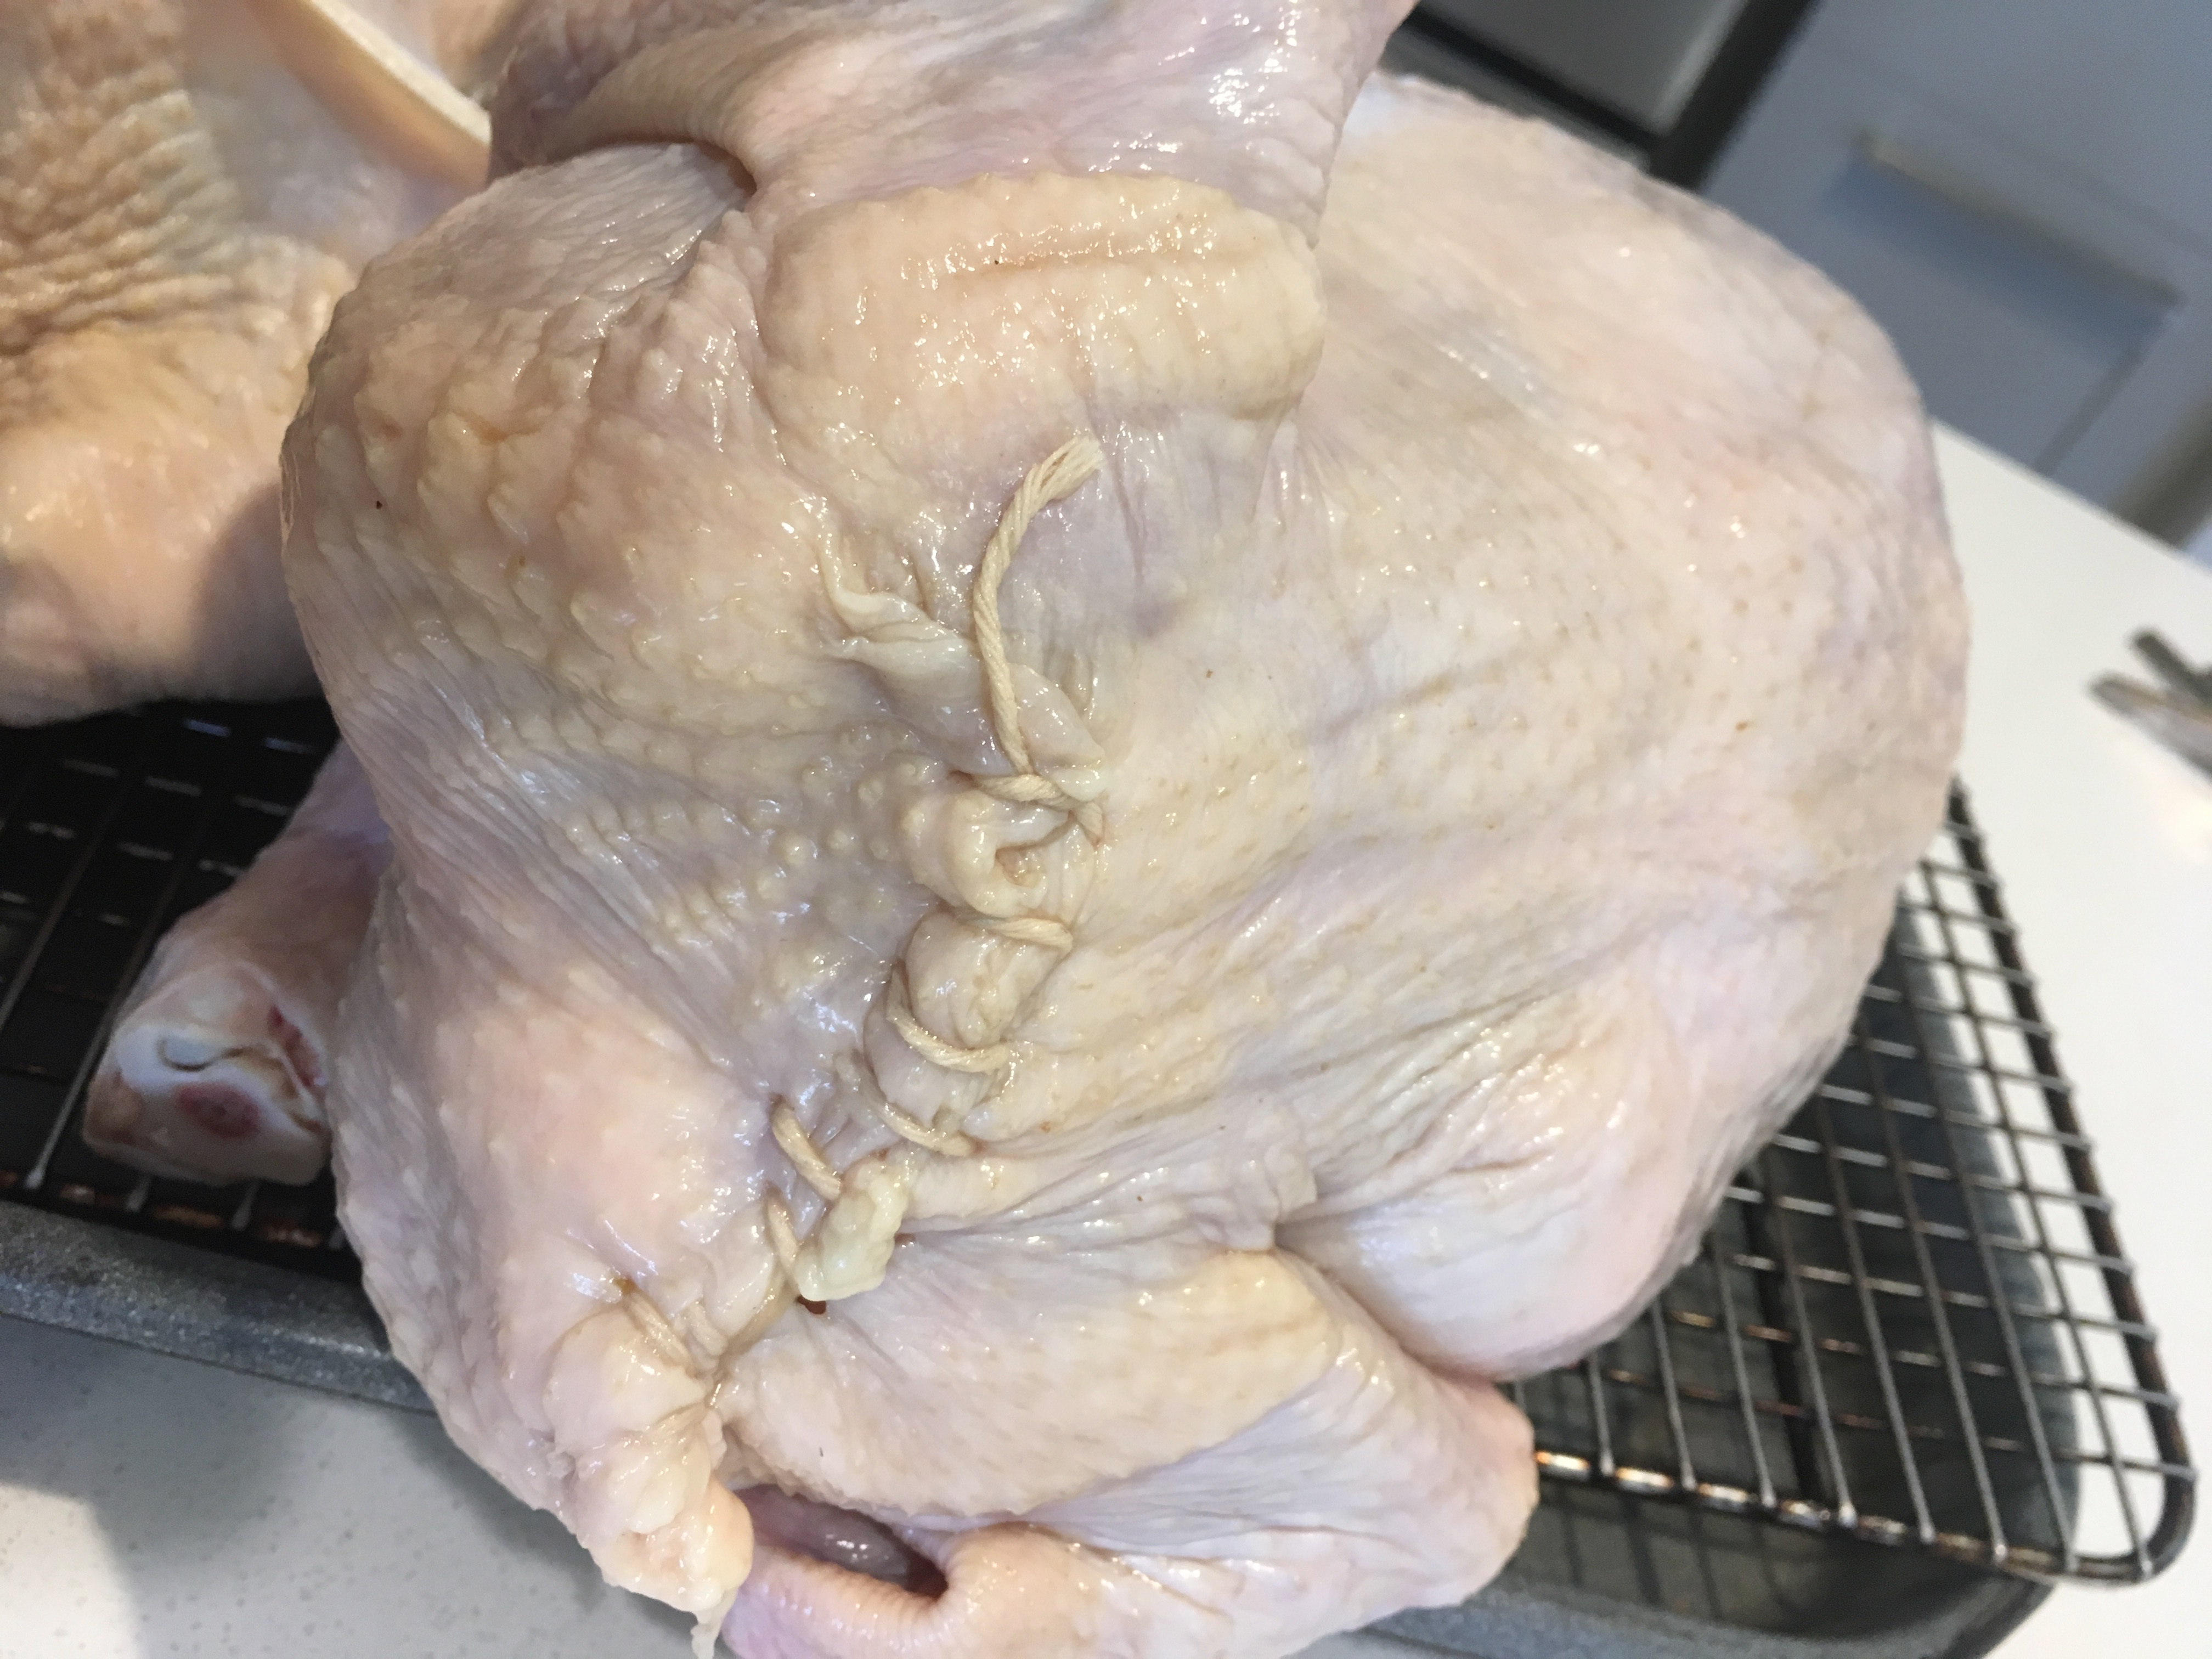
\includegraphics[width=0.25\textwidth]{\imageDir/\fileName/IMG_3218.jpg} &
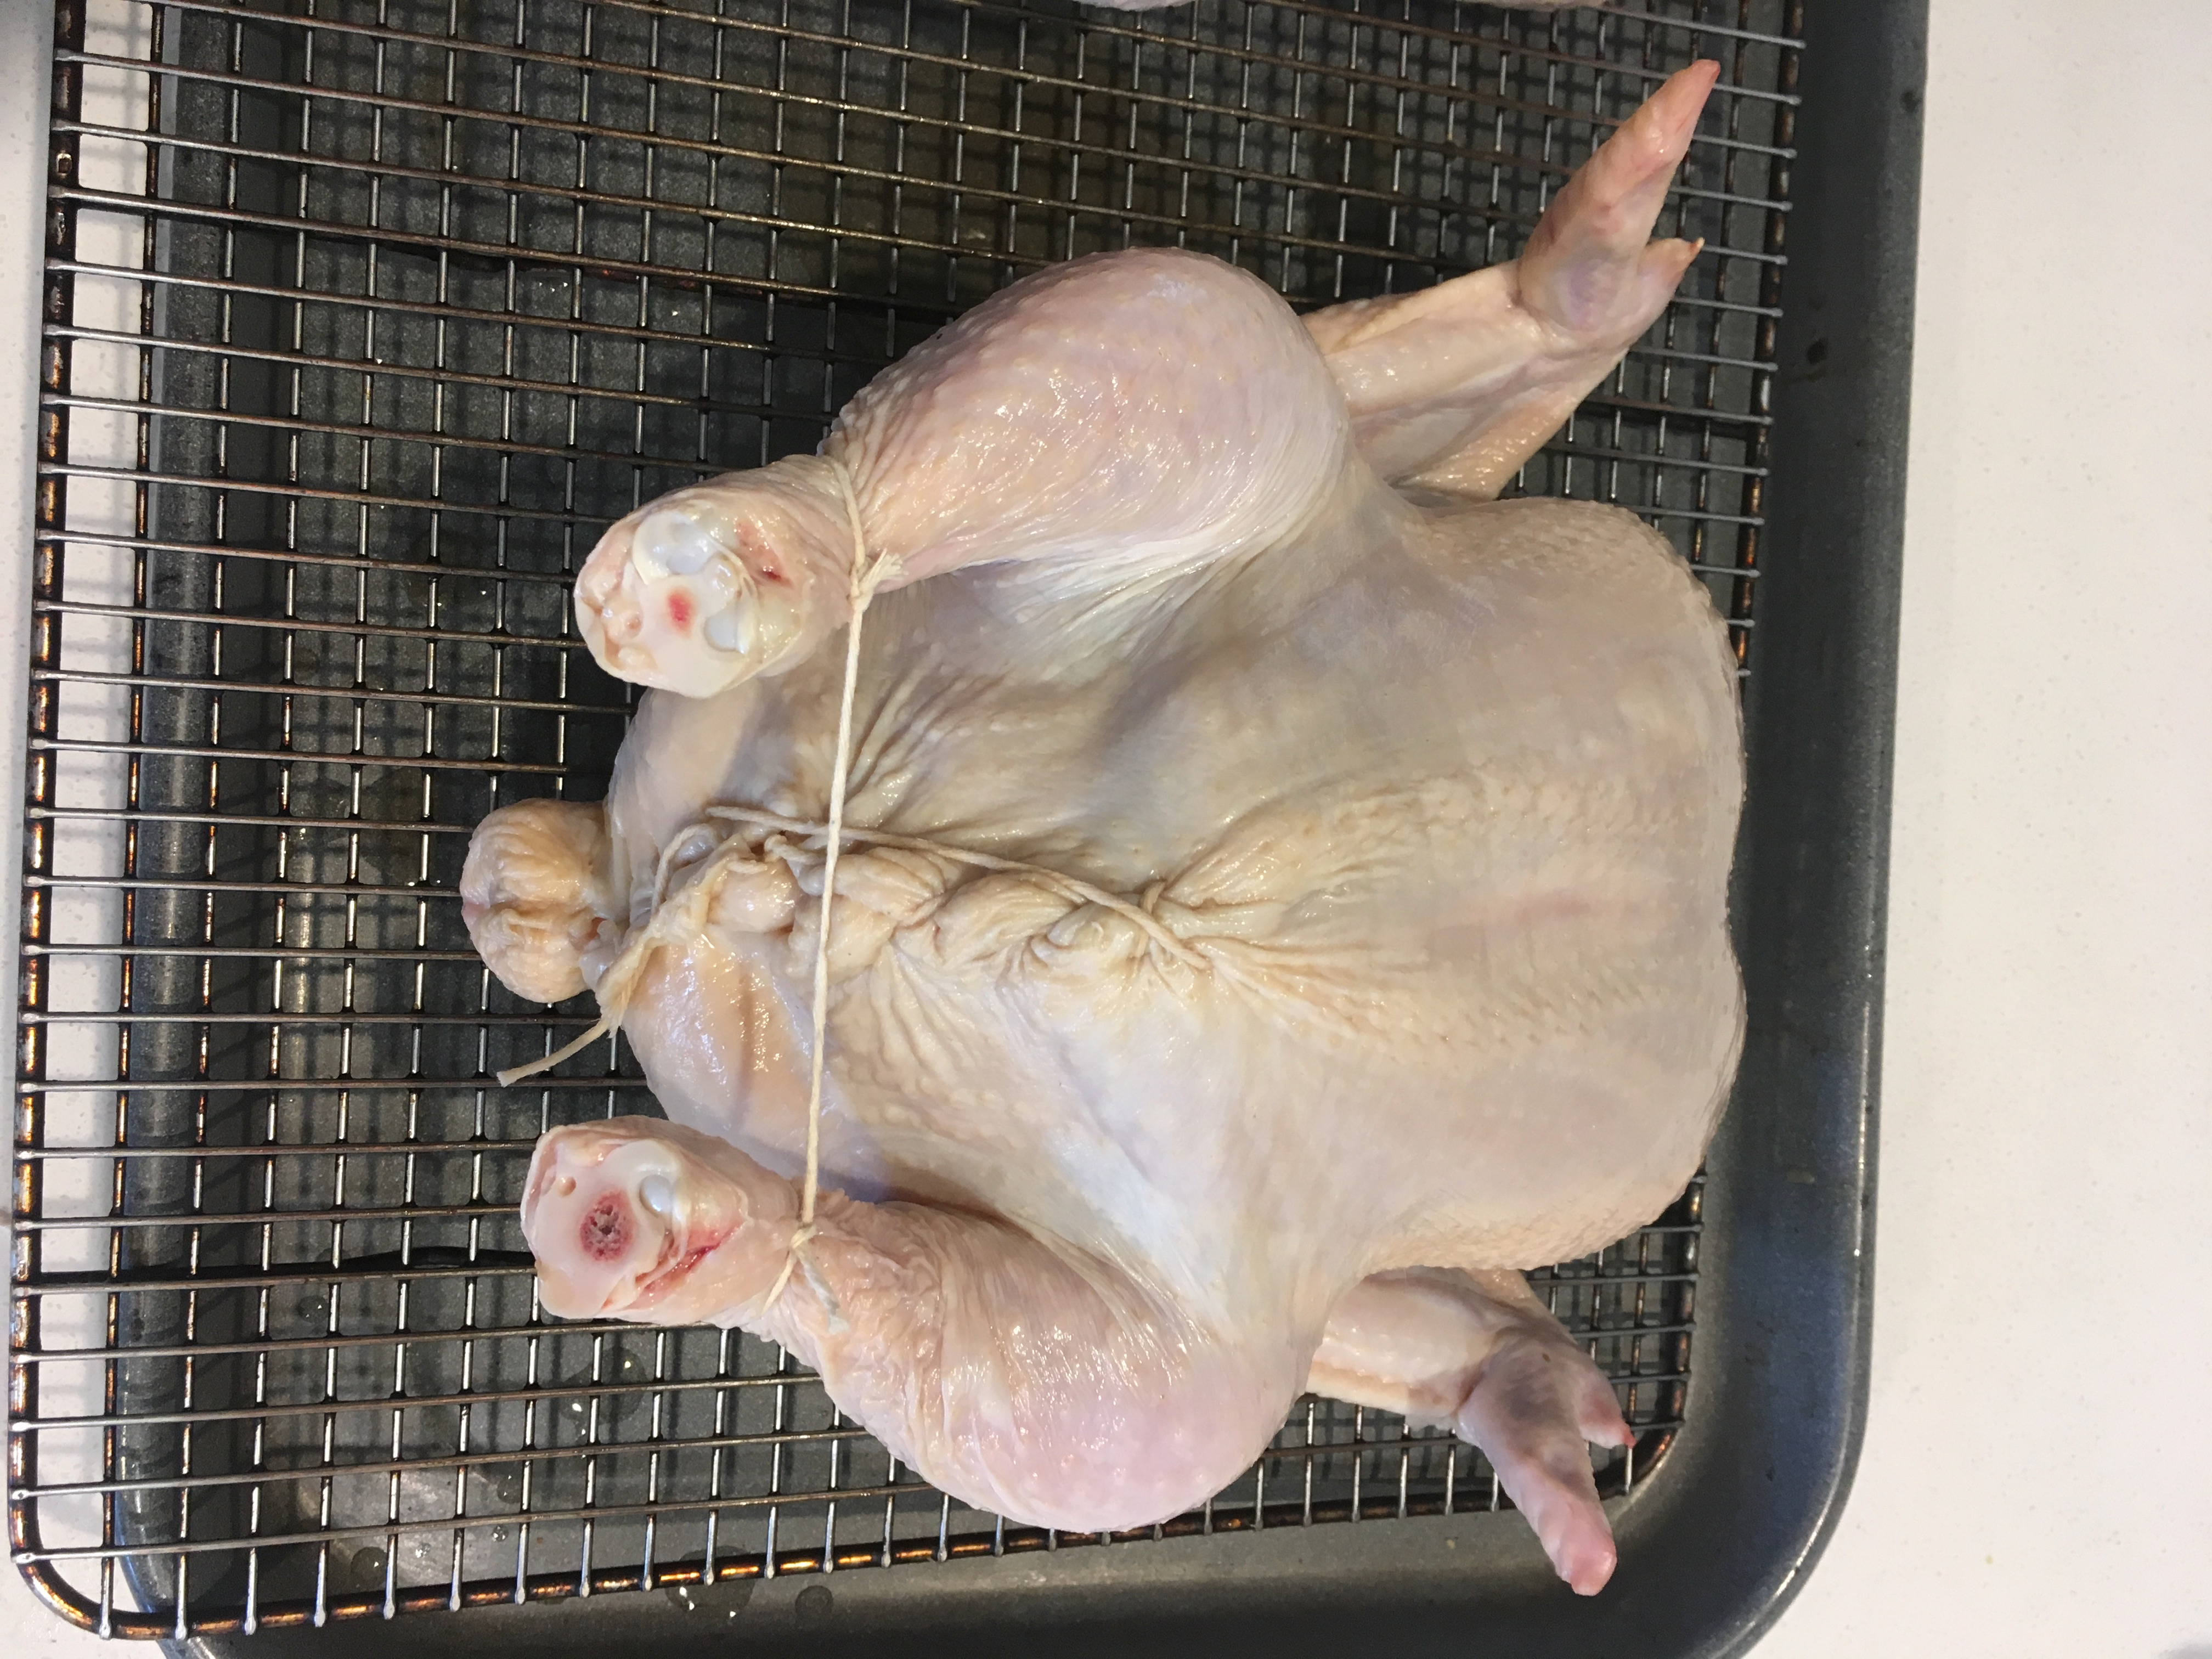
\includegraphics[width=0.25\textwidth]{\imageDir/\fileName/IMG_3219.jpg} \\
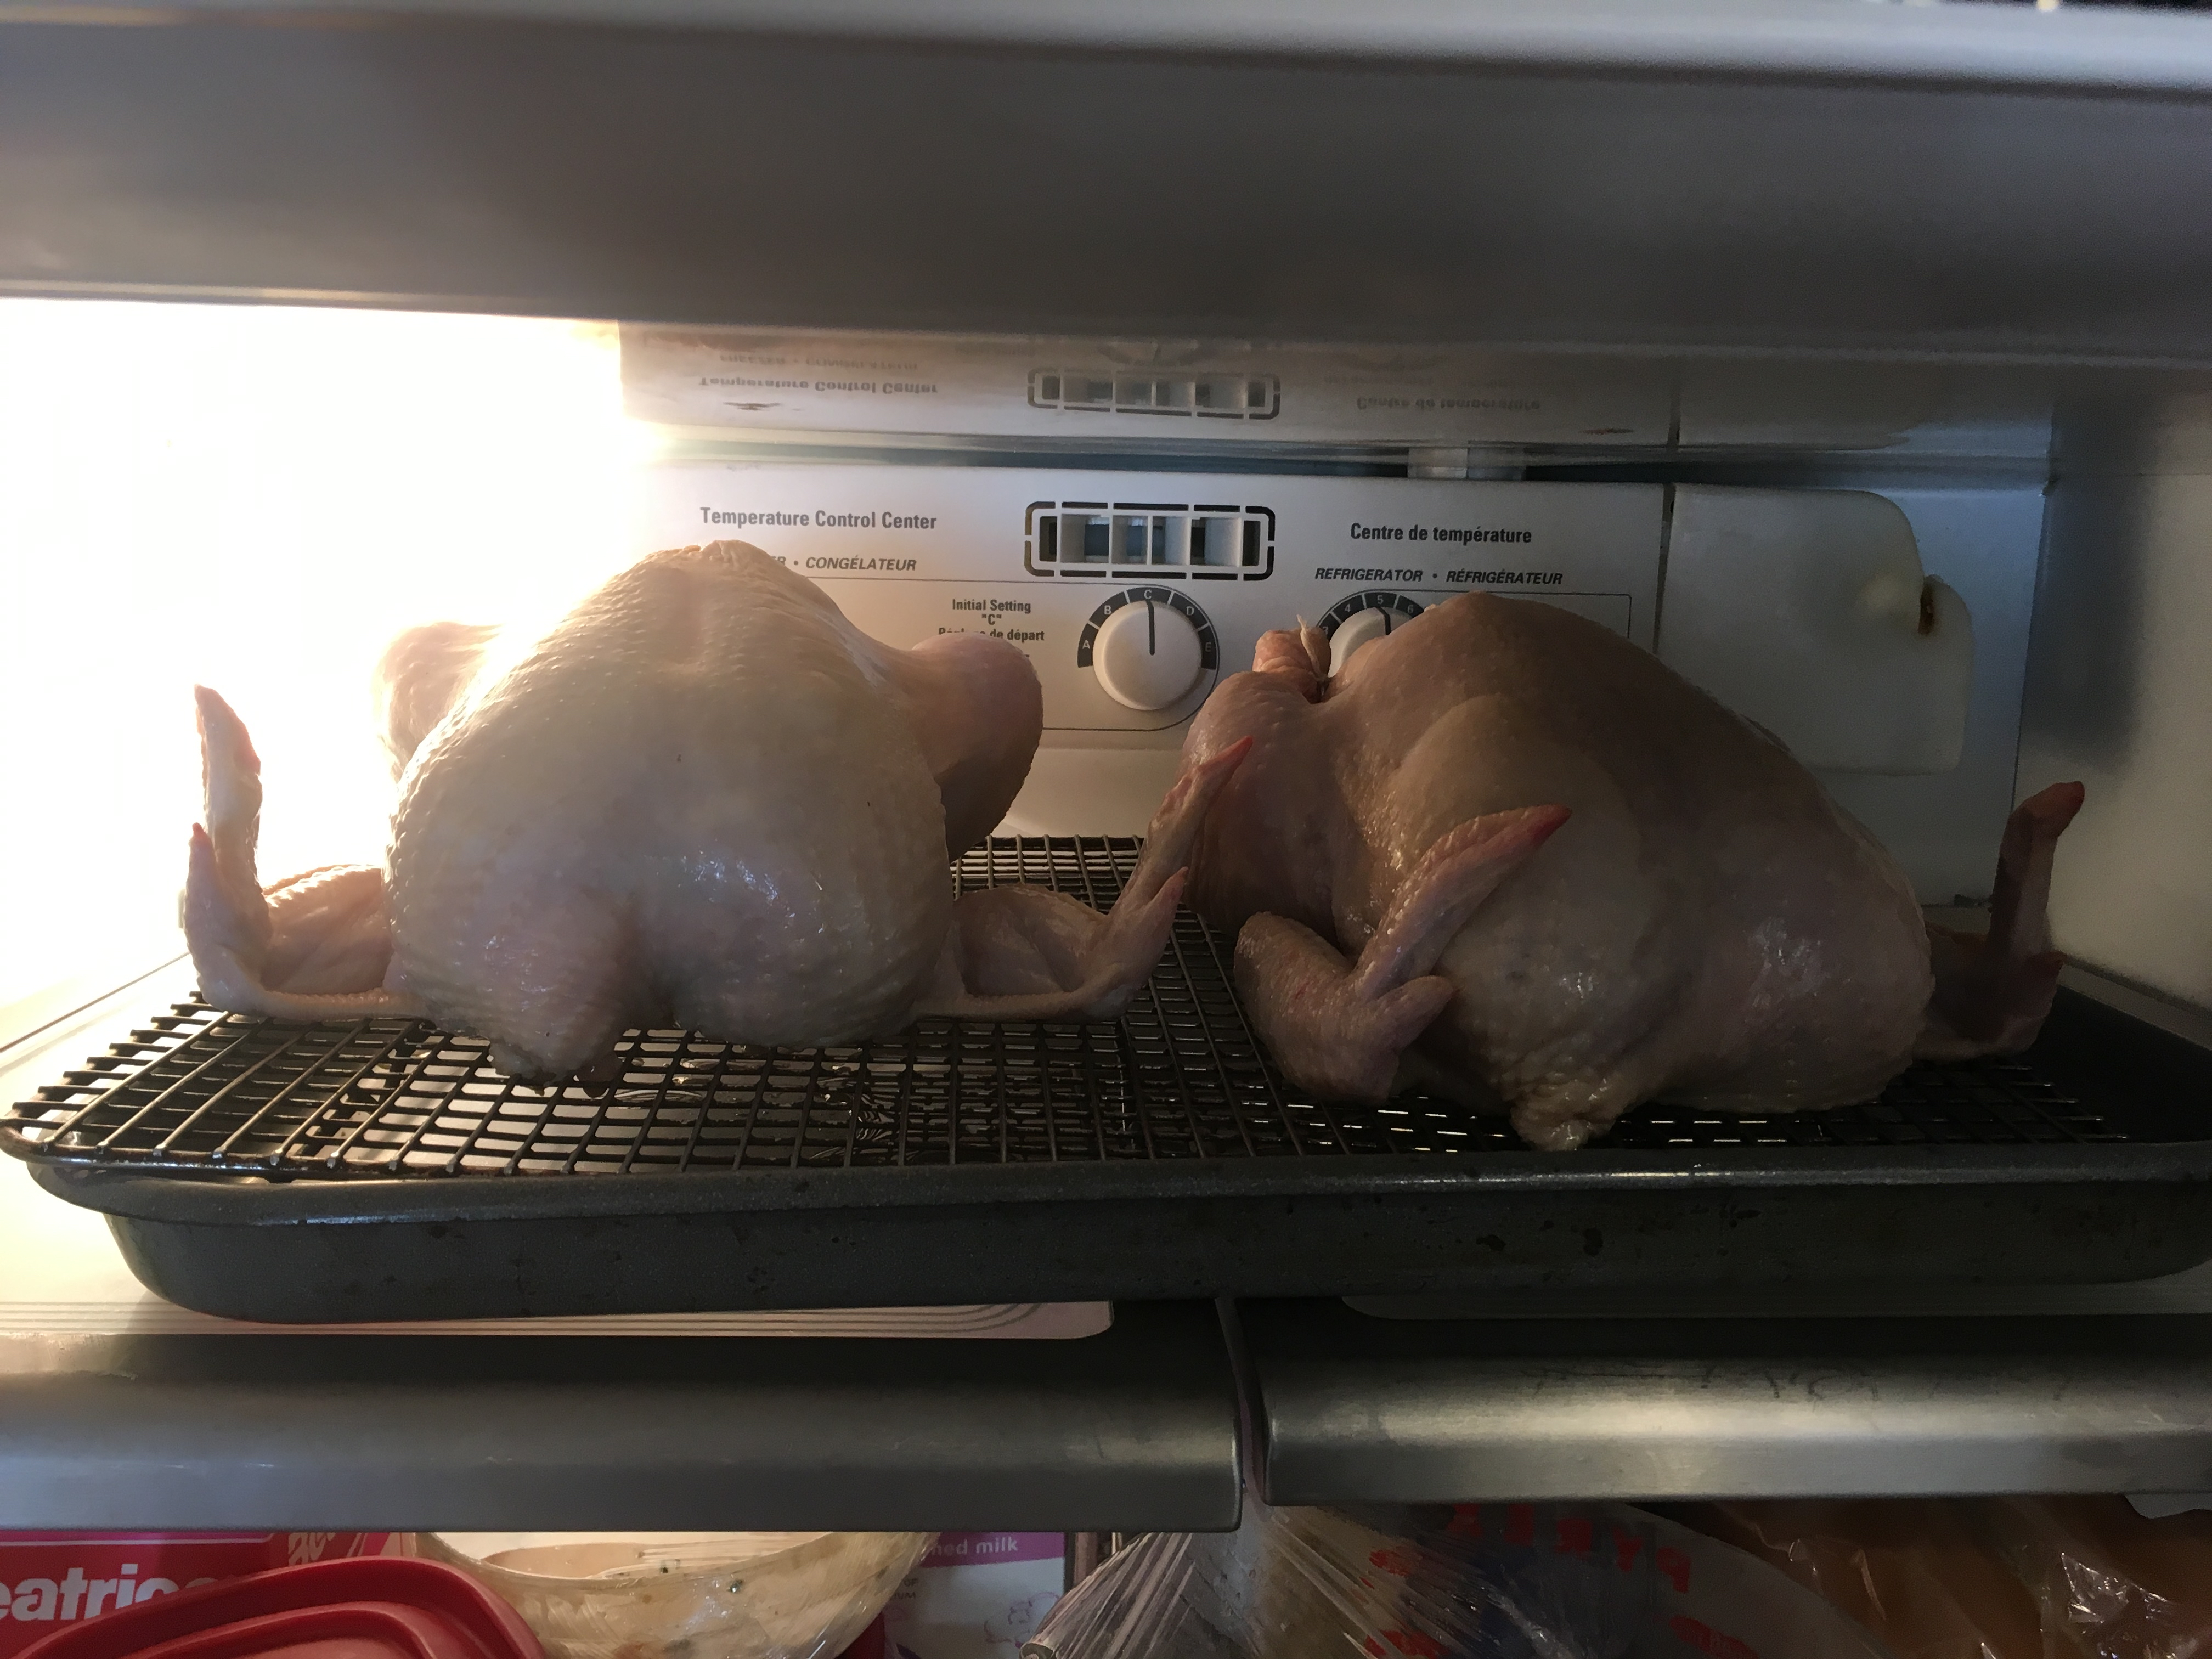
\includegraphics[width=0.25\textwidth]{\imageDir/\fileName/IMG_3220.jpg} &
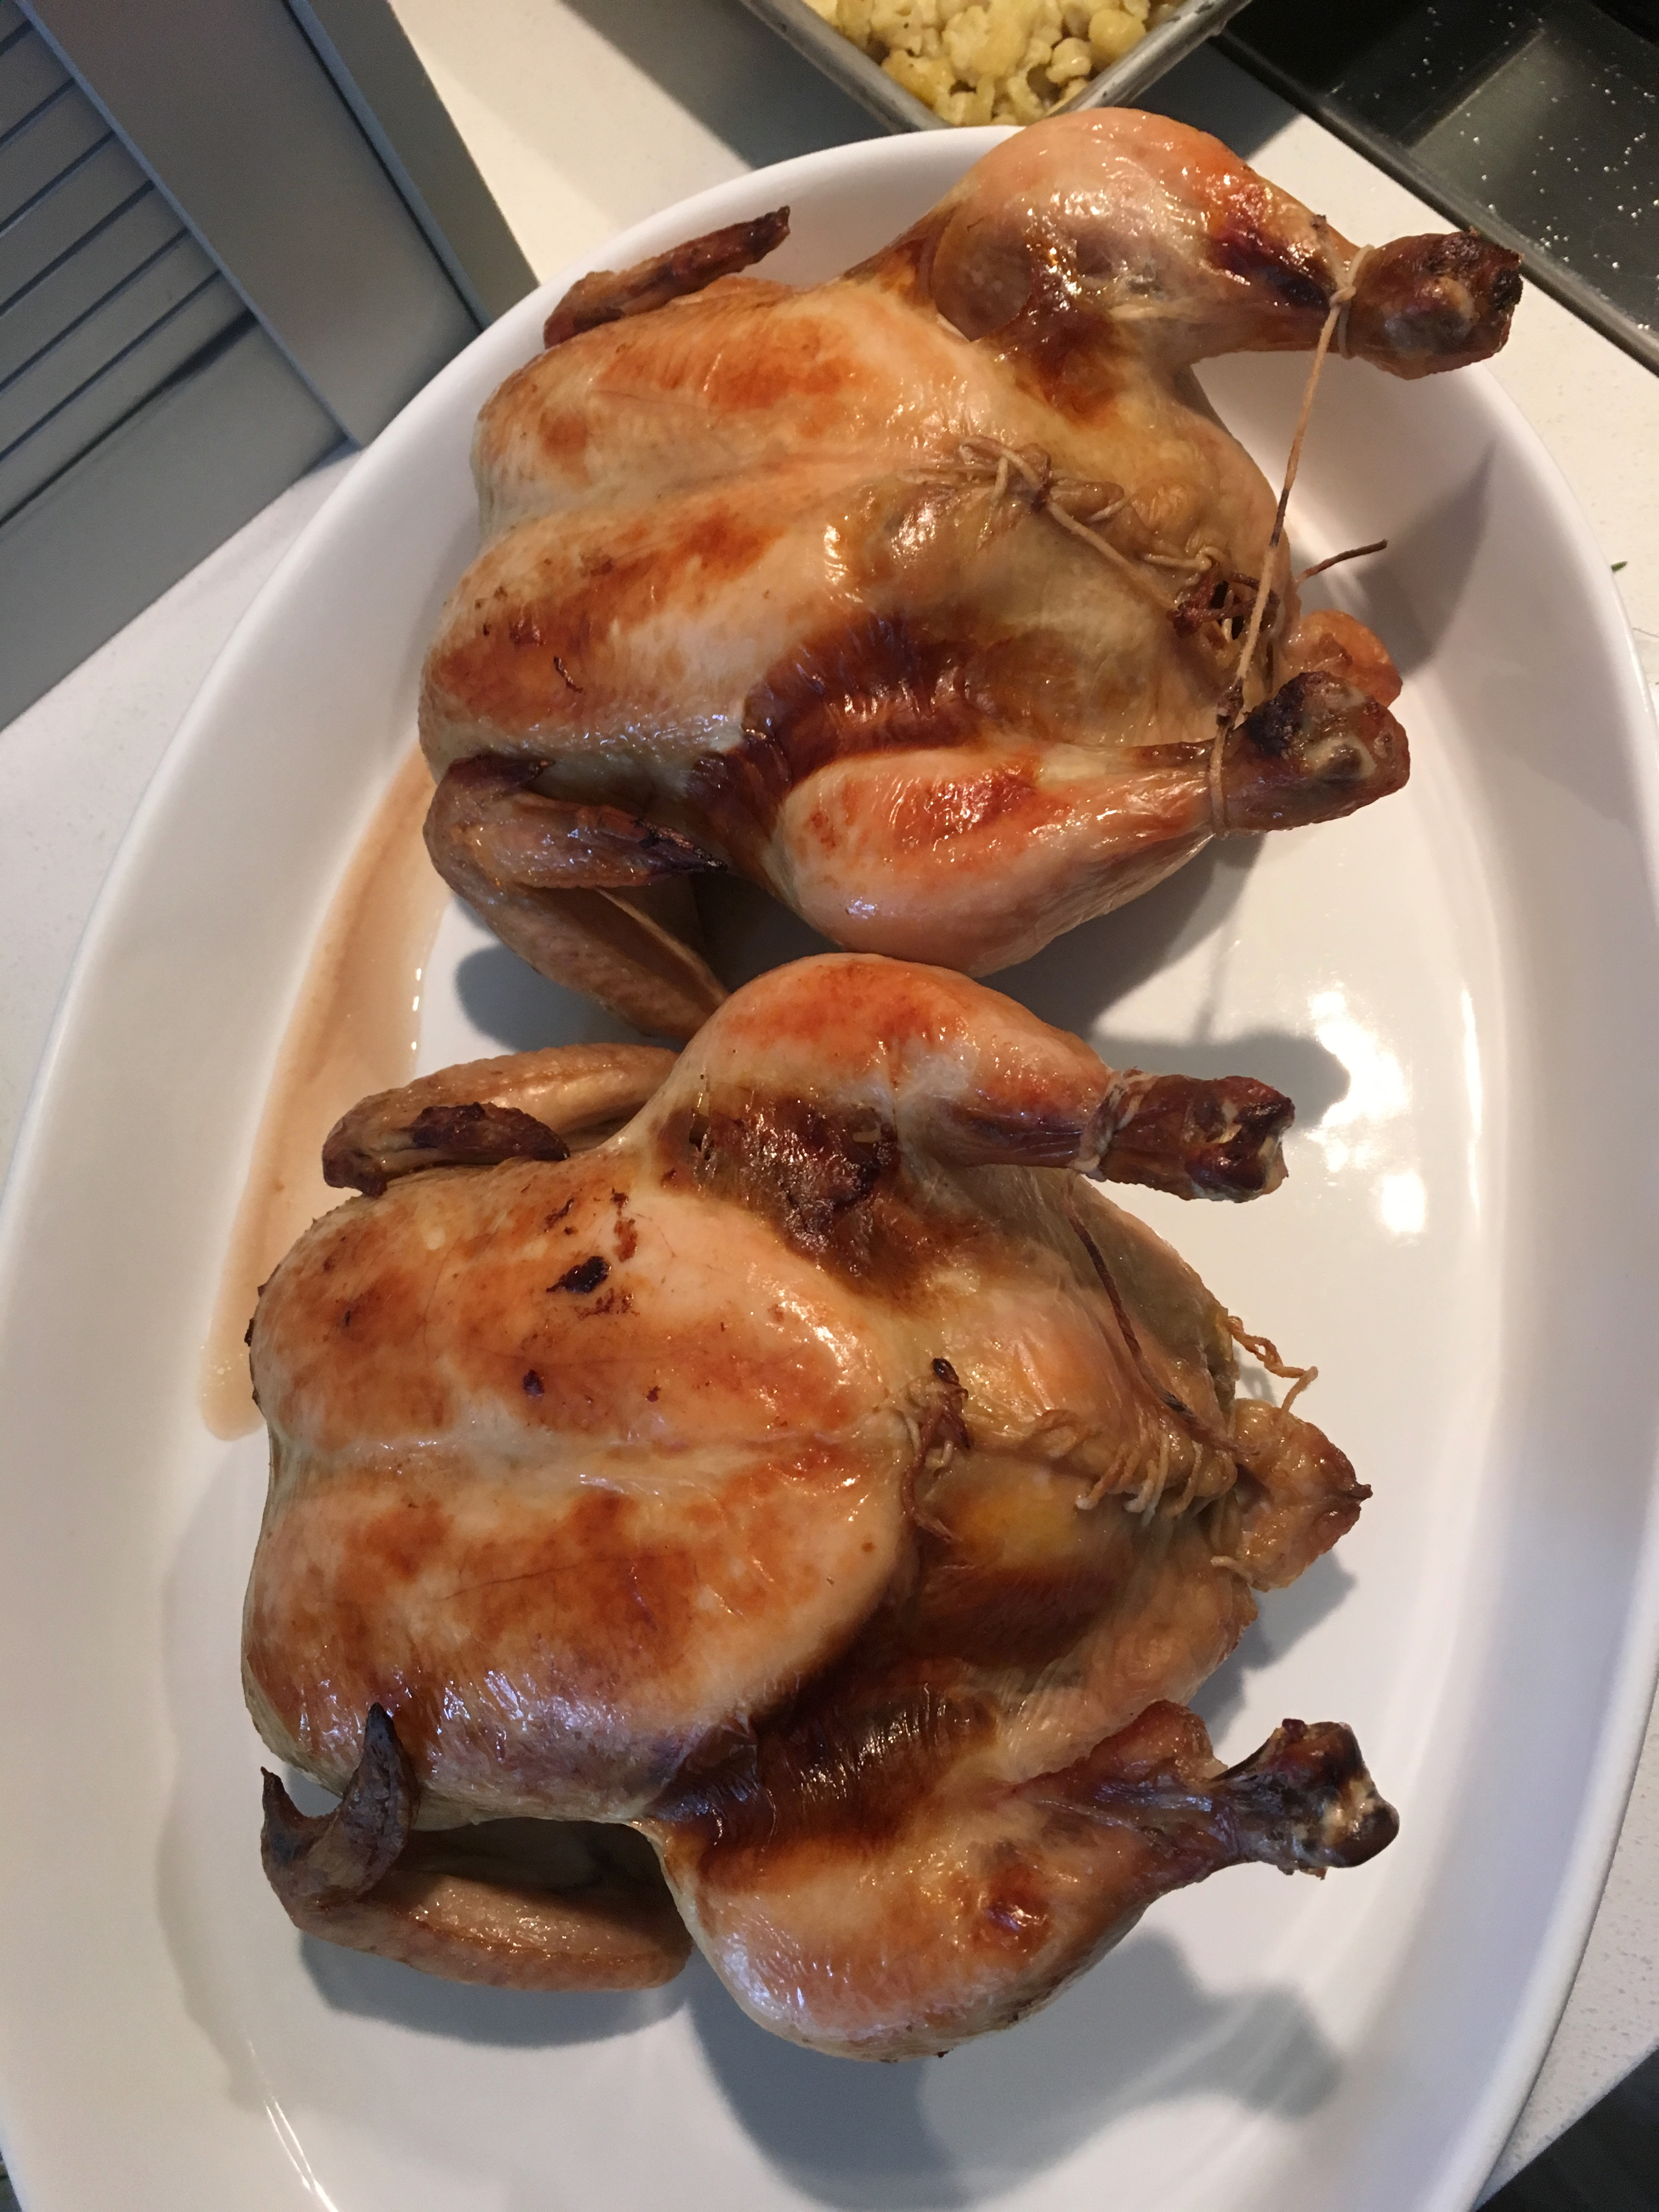
\includegraphics[width=0.25\textwidth]{\imageDir/\fileName/IMG_3228.jpg} \\
\end{tabular}
\end{table}

\end{document}
